\documentclass[]{article}
\usepackage{lmodern}
\usepackage{amssymb,amsmath}
\usepackage{ifxetex,ifluatex}
\usepackage{fixltx2e} % provides \textsubscript
\ifnum 0\ifxetex 1\fi\ifluatex 1\fi=0 % if pdftex
  \usepackage[T1]{fontenc}
  \usepackage[utf8]{inputenc}
\else % if luatex or xelatex
  \ifxetex
    \usepackage{mathspec}
  \else
    \usepackage{fontspec}
  \fi
  \defaultfontfeatures{Ligatures=TeX,Scale=MatchLowercase}
\fi
% use upquote if available, for straight quotes in verbatim environments
\IfFileExists{upquote.sty}{\usepackage{upquote}}{}
% use microtype if available
\IfFileExists{microtype.sty}{%
\usepackage{microtype}
\UseMicrotypeSet[protrusion]{basicmath} % disable protrusion for tt fonts
}{}
\usepackage[margin=1in]{geometry}
\usepackage{hyperref}
\hypersetup{unicode=true,
            pdftitle={Suffolk 2019},
            pdfborder={0 0 0},
            breaklinks=true}
\urlstyle{same}  % don't use monospace font for urls
\usepackage{color}
\usepackage{fancyvrb}
\newcommand{\VerbBar}{|}
\newcommand{\VERB}{\Verb[commandchars=\\\{\}]}
\DefineVerbatimEnvironment{Highlighting}{Verbatim}{commandchars=\\\{\}}
% Add ',fontsize=\small' for more characters per line
\usepackage{framed}
\definecolor{shadecolor}{RGB}{248,248,248}
\newenvironment{Shaded}{\begin{snugshade}}{\end{snugshade}}
\newcommand{\AlertTok}[1]{\textcolor[rgb]{0.94,0.16,0.16}{#1}}
\newcommand{\AnnotationTok}[1]{\textcolor[rgb]{0.56,0.35,0.01}{\textbf{\textit{#1}}}}
\newcommand{\AttributeTok}[1]{\textcolor[rgb]{0.77,0.63,0.00}{#1}}
\newcommand{\BaseNTok}[1]{\textcolor[rgb]{0.00,0.00,0.81}{#1}}
\newcommand{\BuiltInTok}[1]{#1}
\newcommand{\CharTok}[1]{\textcolor[rgb]{0.31,0.60,0.02}{#1}}
\newcommand{\CommentTok}[1]{\textcolor[rgb]{0.56,0.35,0.01}{\textit{#1}}}
\newcommand{\CommentVarTok}[1]{\textcolor[rgb]{0.56,0.35,0.01}{\textbf{\textit{#1}}}}
\newcommand{\ConstantTok}[1]{\textcolor[rgb]{0.00,0.00,0.00}{#1}}
\newcommand{\ControlFlowTok}[1]{\textcolor[rgb]{0.13,0.29,0.53}{\textbf{#1}}}
\newcommand{\DataTypeTok}[1]{\textcolor[rgb]{0.13,0.29,0.53}{#1}}
\newcommand{\DecValTok}[1]{\textcolor[rgb]{0.00,0.00,0.81}{#1}}
\newcommand{\DocumentationTok}[1]{\textcolor[rgb]{0.56,0.35,0.01}{\textbf{\textit{#1}}}}
\newcommand{\ErrorTok}[1]{\textcolor[rgb]{0.64,0.00,0.00}{\textbf{#1}}}
\newcommand{\ExtensionTok}[1]{#1}
\newcommand{\FloatTok}[1]{\textcolor[rgb]{0.00,0.00,0.81}{#1}}
\newcommand{\FunctionTok}[1]{\textcolor[rgb]{0.00,0.00,0.00}{#1}}
\newcommand{\ImportTok}[1]{#1}
\newcommand{\InformationTok}[1]{\textcolor[rgb]{0.56,0.35,0.01}{\textbf{\textit{#1}}}}
\newcommand{\KeywordTok}[1]{\textcolor[rgb]{0.13,0.29,0.53}{\textbf{#1}}}
\newcommand{\NormalTok}[1]{#1}
\newcommand{\OperatorTok}[1]{\textcolor[rgb]{0.81,0.36,0.00}{\textbf{#1}}}
\newcommand{\OtherTok}[1]{\textcolor[rgb]{0.56,0.35,0.01}{#1}}
\newcommand{\PreprocessorTok}[1]{\textcolor[rgb]{0.56,0.35,0.01}{\textit{#1}}}
\newcommand{\RegionMarkerTok}[1]{#1}
\newcommand{\SpecialCharTok}[1]{\textcolor[rgb]{0.00,0.00,0.00}{#1}}
\newcommand{\SpecialStringTok}[1]{\textcolor[rgb]{0.31,0.60,0.02}{#1}}
\newcommand{\StringTok}[1]{\textcolor[rgb]{0.31,0.60,0.02}{#1}}
\newcommand{\VariableTok}[1]{\textcolor[rgb]{0.00,0.00,0.00}{#1}}
\newcommand{\VerbatimStringTok}[1]{\textcolor[rgb]{0.31,0.60,0.02}{#1}}
\newcommand{\WarningTok}[1]{\textcolor[rgb]{0.56,0.35,0.01}{\textbf{\textit{#1}}}}
\usepackage{longtable,booktabs}
\usepackage{graphicx,grffile}
\makeatletter
\def\maxwidth{\ifdim\Gin@nat@width>\linewidth\linewidth\else\Gin@nat@width\fi}
\def\maxheight{\ifdim\Gin@nat@height>\textheight\textheight\else\Gin@nat@height\fi}
\makeatother
% Scale images if necessary, so that they will not overflow the page
% margins by default, and it is still possible to overwrite the defaults
% using explicit options in \includegraphics[width, height, ...]{}
\setkeys{Gin}{width=\maxwidth,height=\maxheight,keepaspectratio}
\IfFileExists{parskip.sty}{%
\usepackage{parskip}
}{% else
\setlength{\parindent}{0pt}
\setlength{\parskip}{6pt plus 2pt minus 1pt}
}
\setlength{\emergencystretch}{3em}  % prevent overfull lines
\providecommand{\tightlist}{%
  \setlength{\itemsep}{0pt}\setlength{\parskip}{0pt}}
\setcounter{secnumdepth}{5}
% Redefines (sub)paragraphs to behave more like sections
\ifx\paragraph\undefined\else
\let\oldparagraph\paragraph
\renewcommand{\paragraph}[1]{\oldparagraph{#1}\mbox{}}
\fi
\ifx\subparagraph\undefined\else
\let\oldsubparagraph\subparagraph
\renewcommand{\subparagraph}[1]{\oldsubparagraph{#1}\mbox{}}
\fi

%%% Use protect on footnotes to avoid problems with footnotes in titles
\let\rmarkdownfootnote\footnote%
\def\footnote{\protect\rmarkdownfootnote}

%%% Change title format to be more compact
\usepackage{titling}

% Create subtitle command for use in maketitle
\providecommand{\subtitle}[1]{
  \posttitle{
    \begin{center}\large#1\end{center}
    }
}

\setlength{\droptitle}{-2em}

  \title{Suffolk 2019}
    \pretitle{\vspace{\droptitle}\centering\huge}
  \posttitle{\par}
    \author{}
    \preauthor{}\postauthor{}
    \date{}
    \predate{}\postdate{}
  

\begin{document}
\maketitle

{
\setcounter{tocdepth}{2}
\tableofcontents
}
\hypertarget{about-this-course}{%
\section*{About this course}\label{about-this-course}}
\addcontentsline{toc}{section}{About this course}

This course is an introduction R, RStudio and statistics. Our primary aims are to get comfortable working with R and to be able to prepare, manipulate, analyse and visualise data.

\begin{center}\rule{0.5\linewidth}{\linethickness}\end{center}

\hypertarget{introduction-to-r-and-rstudio}{%
\section{Introduction to R and RStudio}\label{introduction-to-r-and-rstudio}}

\hypertarget{learning-objectives}{%
\subsection{Learning objectives}\label{learning-objectives}}

In this session, we will have a look at R and RStudio. We will interact with both and use the various components of RStudio.

\hypertarget{what-is-r}{%
\subsubsection{What is R?}\label{what-is-r}}

R is an environment for statistical computing and graphics. RStudio is an editor or integrated development environment (IDE) that makes working with R much more comfortable.

To install R and RStudio on your computer, download both from the following sources:

\begin{itemize}
\tightlist
\item
  Download R from \href{https://cran.r-project.org}{The Comprehensive R Archive Network (CRAN)}
\item
  Download RStudio from \href{https://www.rstudio.com}{RStudio.com}
\end{itemize}

Keep both R and RStudio up to date. That means go online and check for newer versions. In case there are new versions, download those and re-install.

\hypertarget{rstudio}{%
\subsubsection{RStudio}\label{rstudio}}

Let's get acquainted with R. When you start RStudio for the first time, you'll see three panes:

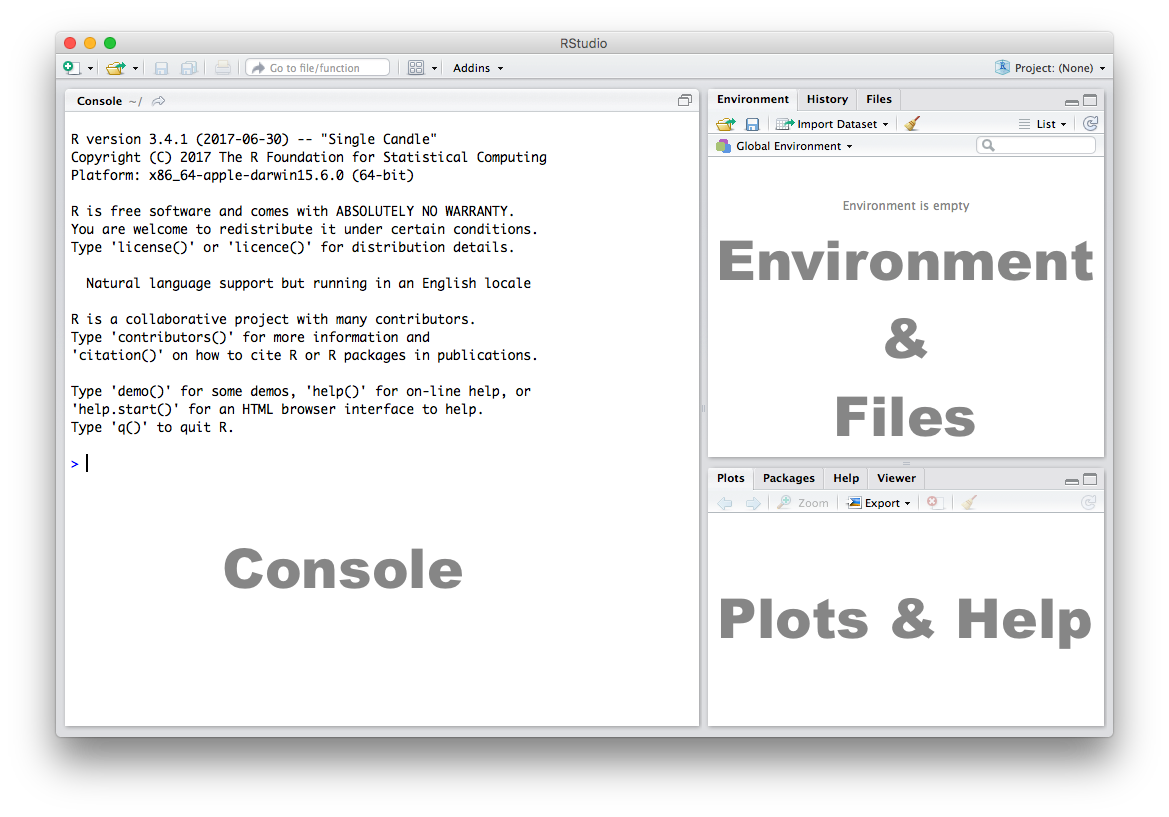
\includegraphics{./img/rstudio_default.png}

\hypertarget{console}{%
\subsubsection{Console}\label{console}}

The Console in RStudio is the simplest way to interact with R. You can type some code at the Console and when you press ENTER, R will run that code. Depending on what you type, you may see some output in the Console or if you make a mistake, you may get a warning or an error message.

Let's familiarize ourselves with the console by using R as a simple calculator:

\begin{Shaded}
\begin{Highlighting}[]
\DecValTok{2} \OperatorTok{+}\StringTok{ }\DecValTok{4}
\end{Highlighting}
\end{Shaded}

\begin{verbatim}
[1] 6
\end{verbatim}

Now that we know how to use the \texttt{+} sign for addition, let's try some other mathematical operations such as subtraction (\texttt{-}), multiplication (\texttt{*}), and division (\texttt{/}).

\begin{Shaded}
\begin{Highlighting}[]
\DecValTok{10} \OperatorTok{-}\StringTok{ }\DecValTok{4}
\end{Highlighting}
\end{Shaded}

\begin{verbatim}
[1] 6
\end{verbatim}

\begin{Shaded}
\begin{Highlighting}[]
\DecValTok{5} \OperatorTok{*}\StringTok{ }\DecValTok{3}
\end{Highlighting}
\end{Shaded}

\begin{verbatim}
[1] 15
\end{verbatim}

\begin{Shaded}
\begin{Highlighting}[]
\DecValTok{7} \OperatorTok{/}\StringTok{ }\DecValTok{2}
\end{Highlighting}
\end{Shaded}

\begin{verbatim}
[1] 3.5
\end{verbatim}

\begin{longtable}[]{@{}ll@{}}
\toprule
\endhead
\begin{minipage}[t]{0.69\columnwidth}\raggedright
You can use the cursor or arrow keys on your keyboard to edit your code at the console:- Use the UP and DOWN keys to re-run something without typing it again- Use the LEFT and RIGHT keys to edit\strut
\end{minipage} & \begin{minipage}[t]{0.25\columnwidth}\raggedright
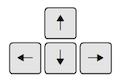
\includegraphics{./img/rstudio_cursorkeys.png}\strut
\end{minipage}\tabularnewline
\bottomrule
\end{longtable}

Take a few minutes to play around at the console and try different things out. Don't worry if you make a mistake, you can't break anything easily!

\hypertarget{scripts}{%
\subsubsection{Scripts}\label{scripts}}

The Console is great for simple tasks but if you're working on a project you would mostly likely want to save your work in some sort of a document or a file. Scripts in R are just plain text files that contain R code. You can edit a script just like you would edit a file in any word processing or note-taking application.

Create a new script using the menu or the toolbar button as shown below.

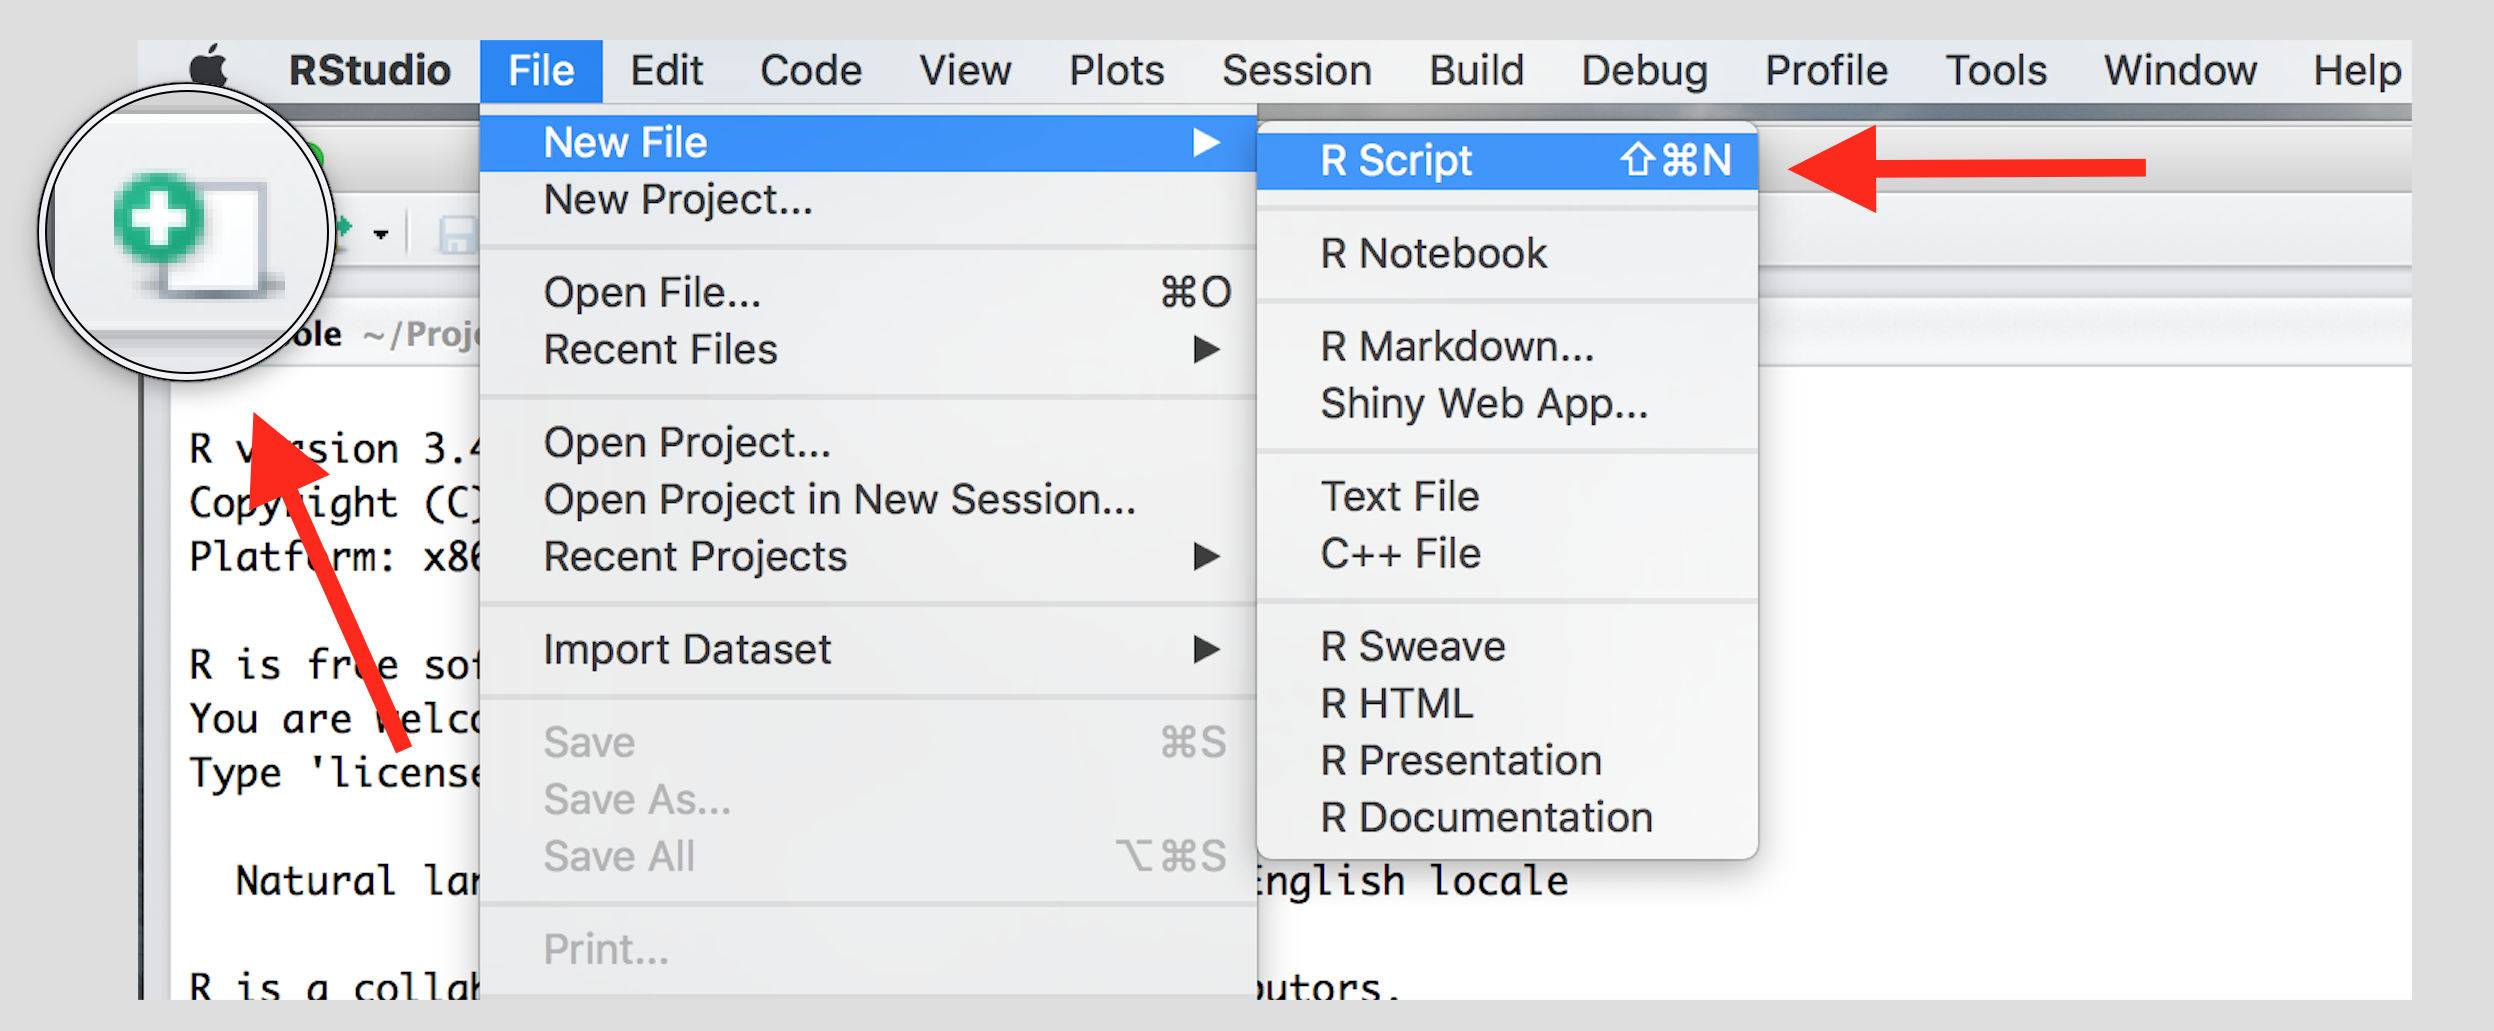
\includegraphics{./img/rstudio_newfile.png}

Once you've created a script, it is generally a good idea to give it a meaningful name and save it immediately. For our first session save your script as \textbf{seminar1.R}

\begin{longtable}[]{@{}ll@{}}
\toprule
\endhead
\begin{minipage}[t]{0.52\columnwidth}\raggedright
Familiarize yourself with the script window in RStudio, and especially the two buttons labeled \textbf{Run} and \textbf{Source}\strut
\end{minipage} & \begin{minipage}[t]{0.42\columnwidth}\raggedright
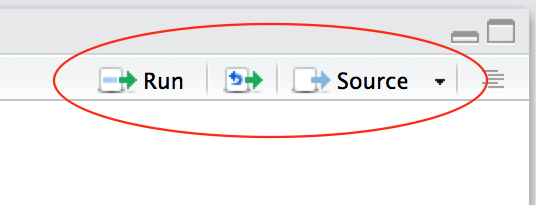
\includegraphics{./img/rstudio_script.png}\strut
\end{minipage}\tabularnewline
\bottomrule
\end{longtable}

There are a few different ways to run your code from a script.

\begin{longtable}[]{@{}ll@{}}
\toprule
\endhead
\begin{minipage}[t]{0.23\columnwidth}\raggedright
One line at a time\strut
\end{minipage} & \begin{minipage}[t]{0.71\columnwidth}\raggedright
Place the cursor on the line you want to run and hit CTRL-ENTER or use the \textbf{Run} button\strut
\end{minipage}\tabularnewline
\begin{minipage}[t]{0.23\columnwidth}\raggedright
Multiple lines\strut
\end{minipage} & \begin{minipage}[t]{0.71\columnwidth}\raggedright
Select the lines you want to run and hit CTRL-ENTER or use the \textbf{Run} button\strut
\end{minipage}\tabularnewline
\begin{minipage}[t]{0.23\columnwidth}\raggedright
Entire script\strut
\end{minipage} & \begin{minipage}[t]{0.71\columnwidth}\raggedright
Use the \textbf{Source} button\strut
\end{minipage}\tabularnewline
\bottomrule
\end{longtable}

\hypertarget{r-syntax-data-structures-and-types}{%
\section{R-syntax, data structures and types}\label{r-syntax-data-structures-and-types}}

\hypertarget{seminar}{%
\subsection{Seminar}\label{seminar}}

In this session we introduce R-syntax, and data types.

\hypertarget{functions}{%
\subsubsection{Functions}\label{functions}}

Functions are a set of instructions that carry out a specific task. Functions often require some input and generate some output. For example, instead of using the \texttt{+} operator for addition, we can use the \texttt{sum} function to add two or more numbers.

\begin{Shaded}
\begin{Highlighting}[]
\KeywordTok{sum}\NormalTok{(}\DecValTok{1}\NormalTok{, }\DecValTok{4}\NormalTok{, }\DecValTok{10}\NormalTok{)}
\end{Highlighting}
\end{Shaded}

\begin{verbatim}
[1] 15
\end{verbatim}

In the example above, \texttt{1,\ 4,\ 10} are the inputs and 15 is the output. A function always requires the use of parenthesis or round brackets \texttt{()}. Inputs to the function are called \textbf{arguments} and go inside the brackets. The output of a function is displayed on the screen but we can also have the option of saving the result of the output. More on this later.

\hypertarget{getting-help}{%
\subsubsection{Getting Help}\label{getting-help}}

Another useful function in R is \texttt{help} which we can use to display online documentation. For example, if we wanted to know how to use the \texttt{sum} function, we could type \texttt{help(sum)} and look at the online documentation.

\begin{Shaded}
\begin{Highlighting}[]
\KeywordTok{help}\NormalTok{(sum)}
\end{Highlighting}
\end{Shaded}

The question mark \texttt{?} can also be used as a shortcut to access online help.

\begin{Shaded}
\begin{Highlighting}[]
\NormalTok{?sum}
\end{Highlighting}
\end{Shaded}

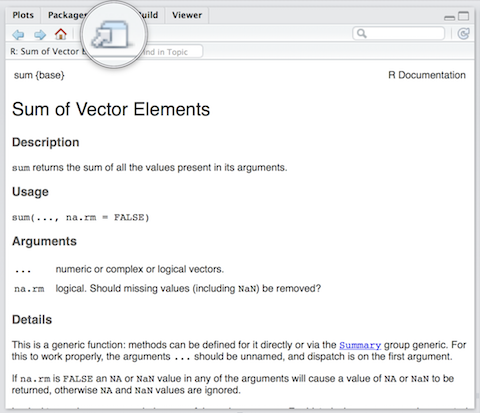
\includegraphics{./img/rstudio_help.png}

Use the toolbar button shown in the picture above to expand and display the help in a new window.

Help pages for functions in R follow a consistent layout generally include these sections:

\begin{longtable}[]{@{}ll@{}}
\toprule
\endhead
Description & A brief description of the function\tabularnewline
Usage & The complete syntax or grammar including all arguments (inputs)\tabularnewline
Arguments & Explanation of each argument\tabularnewline
Details & Any relevant details about the function and its arguments\tabularnewline
Value & The output value of the function\tabularnewline
Examples & Example of how to use the function\tabularnewline
\bottomrule
\end{longtable}

\hypertarget{the-assignment-operator}{%
\subsubsection{The Assignment Operator}\label{the-assignment-operator}}

Now we know how to provide inputs to a function using parenthesis or round brackets \texttt{()}, but what about the output of a function?

We use the assignment operator \textbf{\texttt{\textless{}-}} for creating or updating objects. If we wanted to save the result of adding \texttt{sum(1,\ 4,\ 10)}, we would do the following:

\begin{Shaded}
\begin{Highlighting}[]
\NormalTok{myresult <-}\StringTok{ }\KeywordTok{sum}\NormalTok{(}\DecValTok{1}\NormalTok{, }\DecValTok{4}\NormalTok{, }\DecValTok{10}\NormalTok{)}
\end{Highlighting}
\end{Shaded}

The line above creates a new object called \texttt{myresult} in our environment and saves the result of the \texttt{sum(1,\ 4,\ 10)} in it. To see what's in \texttt{myresult}, just type it at the console:

\begin{Shaded}
\begin{Highlighting}[]
\NormalTok{myresult}
\end{Highlighting}
\end{Shaded}

\begin{verbatim}
[1] 15
\end{verbatim}

Take a look at the \textbf{Environment} pane in RStudio and you'll see \texttt{myresult} there.

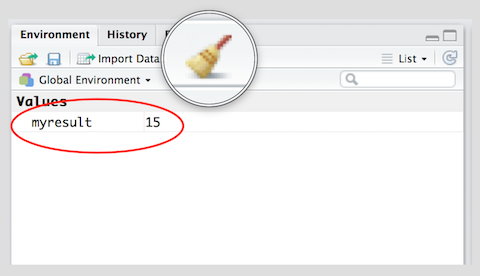
\includegraphics{./img/rstudio_env.png}

To delete all objects from the environment, you can use the \textbf{broom} button as shown in the picture above.

We called our object \texttt{myresult} but we can call it anything as long as we follow a few simple rules. Object names can contain upper or lower case letters (\texttt{A-Z}, \texttt{a-z}), numbers (\texttt{0-9}), underscores (\texttt{\_}) or a dot (\texttt{.}) but all object names must start with a letter. Choose names that are descriptive and easy to type.

\begin{longtable}[]{@{}ll@{}}
\toprule
Good Object Names & Bad Object Names\tabularnewline
\midrule
\endhead
result & a\tabularnewline
myresult & x1\tabularnewline
my.result & this.name.is.just.too.long\tabularnewline
my\_result &\tabularnewline
data1 &\tabularnewline
\bottomrule
\end{longtable}

\hypertarget{vectors-and-subsetting}{%
\subsubsection{Vectors and subsetting}\label{vectors-and-subsetting}}

A vector is one dimensional. It can contain one element in which case it is also called a scalar or many elements. We can add and multiply vectors. Think of a vector as a row or column in your excel spreadsheet.

To create a vector, we use the \texttt{c()} function, where c stands for collect. We start by creating a numeric vector.

\begin{Shaded}
\begin{Highlighting}[]
\NormalTok{vec1 <-}\StringTok{ }\KeywordTok{c}\NormalTok{(}\DecValTok{10}\NormalTok{, }\DecValTok{47}\NormalTok{, }\DecValTok{99}\NormalTok{, }\DecValTok{34}\NormalTok{, }\DecValTok{21}\NormalTok{)}
\end{Highlighting}
\end{Shaded}

Creating a character vector works in the same way. We need to use quotation marks to indicate that the data type is textual data.

\begin{Shaded}
\begin{Highlighting}[]
\NormalTok{vec2 <-}\StringTok{ }\KeywordTok{c}\NormalTok{(}\StringTok{"Emilia"}\NormalTok{, }\StringTok{"Martin"}\NormalTok{, }\StringTok{"Agatha"}\NormalTok{, }\StringTok{"James"}\NormalTok{, }\StringTok{"Luke"}\NormalTok{, }\StringTok{"Jacques"}\NormalTok{)}
\end{Highlighting}
\end{Shaded}

Let's see how many elements our vector contains using the \texttt{length()} function.

\begin{Shaded}
\begin{Highlighting}[]
\KeywordTok{length}\NormalTok{(vec1)}
\end{Highlighting}
\end{Shaded}

\begin{verbatim}
[1] 5
\end{verbatim}

\begin{Shaded}
\begin{Highlighting}[]
\KeywordTok{length}\NormalTok{(vec2)}
\end{Highlighting}
\end{Shaded}

\begin{verbatim}
[1] 6
\end{verbatim}

We need one coordinate to identify a unique element in a vector. For instance, we may be interested in the first element of the vector only. We use square brackets \texttt{{[}{]}} to access a specific element. The number in square brackets is the vector element that we wish to see.

\begin{Shaded}
\begin{Highlighting}[]
\NormalTok{vec1[}\DecValTok{1}\NormalTok{]}
\end{Highlighting}
\end{Shaded}

\begin{verbatim}
[1] 10
\end{verbatim}

To access all elements except the first element, we use the \texttt{-} operator

\begin{Shaded}
\begin{Highlighting}[]
\NormalTok{vec1[}\OperatorTok{-}\DecValTok{1}\NormalTok{]}
\end{Highlighting}
\end{Shaded}

\begin{verbatim}
[1] 47 99 34 21
\end{verbatim}

We can access elements 2 to 4 by using the colon \texttt{:} operator.

\begin{Shaded}
\begin{Highlighting}[]
\NormalTok{vec1[}\DecValTok{2}\OperatorTok{:}\DecValTok{4}\NormalTok{]}
\end{Highlighting}
\end{Shaded}

\begin{verbatim}
[1] 47 99 34
\end{verbatim}

We can access non-adjacent elements bu using the collect function \texttt{c()}.

\begin{Shaded}
\begin{Highlighting}[]
\NormalTok{vec1[}\KeywordTok{c}\NormalTok{(}\DecValTok{2}\NormalTok{,}\DecValTok{5}\NormalTok{)]}
\end{Highlighting}
\end{Shaded}

\begin{verbatim}
[1] 47 21
\end{verbatim}

Finally, we combine the \texttt{length()} function with the square brackets to access the last element in our vector.

\begin{Shaded}
\begin{Highlighting}[]
\NormalTok{vec1[ }\KeywordTok{length}\NormalTok{(vec1) ]}
\end{Highlighting}
\end{Shaded}

\begin{verbatim}
[1] 21
\end{verbatim}

\hypertarget{matrices}{%
\subsubsection{Matrices}\label{matrices}}

A matrix has two dimensions and stores data of the same type, e.g.~numbers or text but never both. A matrix is always rectangular. Think of it as your excel spreadsheet - essentially, it is a data table.

We create a matrix using the \texttt{matrix()} function. We need to provide the following arguments:

\begin{Shaded}
\begin{Highlighting}[]
\NormalTok{mat1 <-}\StringTok{ }\KeywordTok{matrix}\NormalTok{(}
  \DataTypeTok{data =} \KeywordTok{c}\NormalTok{(}\DecValTok{99}\NormalTok{, }\DecValTok{17}\NormalTok{, }\DecValTok{19}\NormalTok{, }\DecValTok{49}\NormalTok{, }\DecValTok{88}\NormalTok{, }\DecValTok{54}\NormalTok{),}
  \DataTypeTok{nrow =} \DecValTok{2}\NormalTok{,}
  \DataTypeTok{ncol =} \DecValTok{3}\NormalTok{,}
  \DataTypeTok{byrow =} \OtherTok{TRUE}
\NormalTok{)}
\end{Highlighting}
\end{Shaded}

\begin{longtable}[]{@{}ll@{}}
\toprule
Argument & Description\tabularnewline
\midrule
\endhead
data & the data in the matrix\tabularnewline
nrow & number of rows\tabularnewline
ncol & number of columns\tabularnewline
byrow & TRUE = matrix is filled rowwise\tabularnewline
\bottomrule
\end{longtable}

To display the matrix, we simply call the object by its name (in this case mat1).

\begin{Shaded}
\begin{Highlighting}[]
\NormalTok{mat1}
\end{Highlighting}
\end{Shaded}

\begin{verbatim}
     [,1] [,2] [,3]
[1,]   99   17   19
[2,]   49   88   54
\end{verbatim}

To access a unique element in a matrix, we need 2 coordinates. First, a row coordinate and second, a column coordinate. We use square brackets and separate the coordinates with a comma \texttt{{[}\ ,\ {]}}. The row coordinate goes before the comma and the column coordinate after.

We can access the the second row and third column like so:

\begin{Shaded}
\begin{Highlighting}[]
\NormalTok{mat1[}\DecValTok{2}\NormalTok{, }\DecValTok{3}\NormalTok{]}
\end{Highlighting}
\end{Shaded}

\begin{verbatim}
[1] 54
\end{verbatim}

To display an entire column, we specify the column we want to display and leave the row coordinate empty like so:

\begin{Shaded}
\begin{Highlighting}[]
\CommentTok{# display the 2nd column}
\NormalTok{mat1[ , }\DecValTok{2}\NormalTok{]}
\end{Highlighting}
\end{Shaded}

\begin{verbatim}
[1] 17 88
\end{verbatim}

Similarly, to display the entire second row, we specify the row coordinate but leave the column coordinate empty.

\begin{Shaded}
\begin{Highlighting}[]
\NormalTok{mat1[}\DecValTok{2}\NormalTok{, ]}
\end{Highlighting}
\end{Shaded}

\begin{verbatim}
[1] 49 88 54
\end{verbatim}

\hypertarget{arrays}{%
\subsubsection{Arrays}\label{arrays}}

Arrays are similar to matrices but can contain more dimensions. You can think of an array as stacking multiple matrices. Generally, we refer to the rows, columns and layers in array. Let's create an array with 2 rows, 3 columns and 4 layers using the \texttt{array()} function.

\begin{Shaded}
\begin{Highlighting}[]
\NormalTok{arr1 <-}\StringTok{ }\KeywordTok{array}\NormalTok{(}
  \DataTypeTok{data =} \KeywordTok{c}\NormalTok{(}\DecValTok{1}\OperatorTok{:}\DecValTok{24}\NormalTok{),}
  \DataTypeTok{dim =} \KeywordTok{c}\NormalTok{(}\DecValTok{2}\NormalTok{, }\DecValTok{3}\NormalTok{, }\DecValTok{4}\NormalTok{)}
\NormalTok{)}
\end{Highlighting}
\end{Shaded}

To display the object, we call it by its name.

\begin{Shaded}
\begin{Highlighting}[]
\NormalTok{arr1}
\end{Highlighting}
\end{Shaded}

\begin{verbatim}
, , 1

     [,1] [,2] [,3]
[1,]    1    3    5
[2,]    2    4    6

, , 2

     [,1] [,2] [,3]
[1,]    7    9   11
[2,]    8   10   12

, , 3

     [,1] [,2] [,3]
[1,]   13   15   17
[2,]   14   16   18

, , 4

     [,1] [,2] [,3]
[1,]   19   21   23
[2,]   20   22   24
\end{verbatim}

We can subset an array using the square brackets \texttt{{[}{]}}. To access a single element we need as many coordinates as our object has dimensions. Let's check the number of dimensions in our object first.

\begin{Shaded}
\begin{Highlighting}[]
\KeywordTok{dim}\NormalTok{(arr1)}
\end{Highlighting}
\end{Shaded}

\begin{verbatim}
[1] 2 3 4
\end{verbatim}

The \texttt{dim()} function informs us that we have 3 dimensions. The first is of length 2, the second of length 3 and the fourth of length 4.

Access the second column of the third layer on your own.

\begin{Shaded}
\begin{Highlighting}[]
\NormalTok{arr1[ , }\DecValTok{2}\NormalTok{, }\DecValTok{3}\NormalTok{] }
\end{Highlighting}
\end{Shaded}

\begin{verbatim}
[1] 15 16
\end{verbatim}

\hypertarget{data-import-from-csv-txt-and-excel}{%
\section{Data import (from csv, txt, and excel)}\label{data-import-from-csv-txt-and-excel}}

\hypertarget{seminar-1}{%
\subsection{Seminar}\label{seminar-1}}

In this section, we will load data in csv, txt, excel and R format. We will learn how to check and set our working directory.

\hypertarget{setting-up}{%
\subsubsection{Setting up}\label{setting-up}}

We set our working directory. R operates in specific directory (folder) on our computer. We create a folder on where we save our scripts. We name the folder \texttt{suffolk2019}. Let's create the folder on our computers now (in finder on Mac and explorer on Windows).

Now, we set our working directory to the folder, we just created like so:

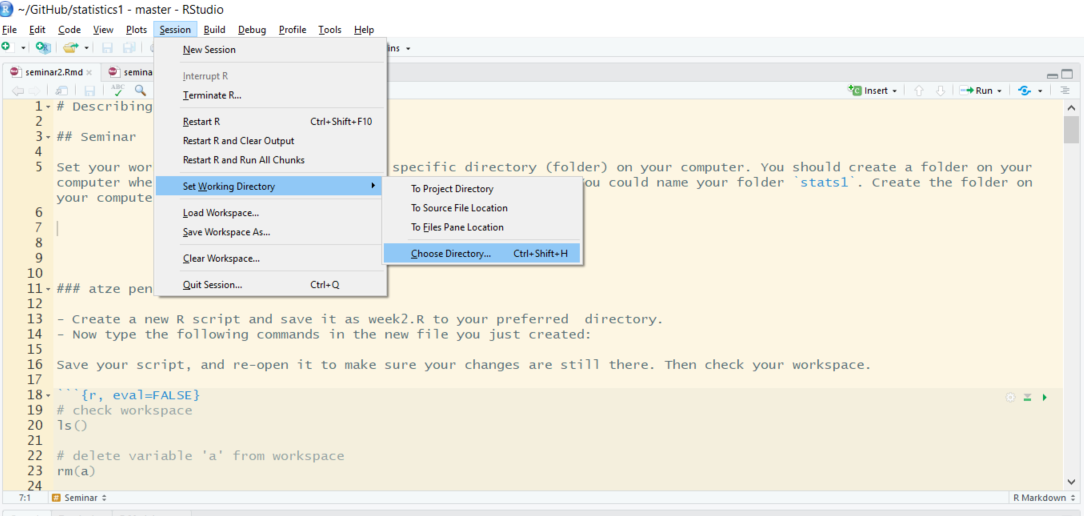
\includegraphics{./img/setwdir.png}

Create a new R script and save it as day1.R to your \texttt{suffolk2019} directory.

At the beginning of each new script, we want to clear the workspace. The workspace is stored in working memory on our computer. If we do not clear it for a new script, it becomes too full over time. Our computer will slow down and it will become difficult for us to know which objects are stored in working memory.

We check the contents of our workspace like so:

\begin{Shaded}
\begin{Highlighting}[]
\CommentTok{# check workspace}
\KeywordTok{ls}\NormalTok{()}
\end{Highlighting}
\end{Shaded}

To remove a specific object, we use the \texttt{rm()} function which stands for remove. Within the round brackets, we put the name of the object we want to remove. We could remove the object \texttt{a} like so:

\begin{Shaded}
\begin{Highlighting}[]
\CommentTok{# delete variable 'a' from workspace}
\KeywordTok{rm}\NormalTok{(a)}
\end{Highlighting}
\end{Shaded}

At the beginning of each script, we should always clear the entire workspace. We can do so in the following way:

\begin{Shaded}
\begin{Highlighting}[]
\CommentTok{# delete everything from workspace}
\KeywordTok{rm}\NormalTok{( }\DataTypeTok{list =} \KeywordTok{ls}\NormalTok{() )}
\end{Highlighting}
\end{Shaded}

You can also clear text from the console window. To do so press Crtl+l on Winowds or Command+l on Mac.

\hypertarget{loading-data}{%
\subsubsection{Loading data}\label{loading-data}}

Data comes in different file formats such as \texttt{.txt}, \texttt{.csv}, \texttt{.xlsx}, \texttt{.RData}, \texttt{.dta} and many more. To know the file type of a file right click on it and view preferences (in Windows explorer or Mac finder).

R can load files coming in many different file formats. To find out how to import a file coming in a specific format, it is usually a good idea to the google ``R load file\_format''.

\hypertarget{importing-a-dataset-in-.csv-format}{%
\subsubsection{\texorpdfstring{Importing a dataset in \texttt{.csv} format}{Importing a dataset in .csv format}}\label{importing-a-dataset-in-.csv-format}}

One of the most common file types is \texttt{.csv} which means comma separated values. Columns are separated by commas and rows by line breaks.

The dataset's name is ``non\_western\_immigrants.csv''. To load it, we use the \texttt{read.csv()} function.

\begin{Shaded}
\begin{Highlighting}[]
\NormalTok{dat1 <-}\StringTok{ }\KeywordTok{read.csv}\NormalTok{(}\StringTok{"non_western_immigrants.csv"}\NormalTok{)}
\end{Highlighting}
\end{Shaded}

\hypertarget{importing-a-dataset-in-excel-xlsx-format}{%
\subsubsection{Importing a dataset in Excel (xlsx) format}\label{importing-a-dataset-in-excel-xlsx-format}}

Another common file format is Microsoft's Excel \texttt{xlsx} format. We will load a dataset in this format now. To do so, we will need to install a package first. Packages are additional functions that we can add to R. A package is like an app on our phones.

We install the \texttt{readxl} package using \texttt{install.packages("readxl")}.

\begin{Shaded}
\begin{Highlighting}[]
\KeywordTok{install.packages}\NormalTok{(}\StringTok{"readxl"}\NormalTok{)}
\end{Highlighting}
\end{Shaded}

We only need to install a package once. It does not hurt to do it more often though, because every time we install, it will install the most recent version of the package.

Once a package is installed, we need to load it using the \texttt{library()} function.

\begin{Shaded}
\begin{Highlighting}[]
\KeywordTok{library}\NormalTok{(readxl)}
\end{Highlighting}
\end{Shaded}

To load the excel file, we can now use the \texttt{read\_excel()} function that is included in the \texttt{readxl} library. We need to provide the following arguments to the function:

\begin{longtable}[]{@{}ll@{}}
\toprule
Argument & Description\tabularnewline
\midrule
\endhead
path & Filename of excel sheet\tabularnewline
sheet & Sheet number to import\tabularnewline
\bottomrule
\end{longtable}

Now, let's load the file:

\begin{Shaded}
\begin{Highlighting}[]
\NormalTok{dat2 <-}\StringTok{ }\KeywordTok{read_excel}\NormalTok{(}\StringTok{"non_western_immigrants.xlsx"}\NormalTok{, }\DataTypeTok{sheet =} \DecValTok{1}\NormalTok{)}
\end{Highlighting}
\end{Shaded}

\hypertarget{importing-a-dataset-in-rdata-format}{%
\subsubsection{Importing a dataset in RData format}\label{importing-a-dataset-in-rdata-format}}

The native file format of R is called \texttt{.RData}. To load files saved in this format, we use the \texttt{load()} function like so:

\begin{Shaded}
\begin{Highlighting}[]
\KeywordTok{load}\NormalTok{(}\DataTypeTok{file =} \StringTok{"non_western_immigrants.RData"}\NormalTok{)}
\end{Highlighting}
\end{Shaded}

Notice that we usually need to assign the object we load to using the \texttt{\textless{}-} operator. The \texttt{load()} function is an exception where we do not need to do this.

\hypertarget{importing-a-dataset-in-.txt-format.}{%
\subsubsection{Importing a dataset in .txt format.}\label{importing-a-dataset-in-.txt-format.}}

Loading a dataset that comes in .txt format requires some additional information. The format is a text format and we need to know how the columns are separated. Usually it is enough to open the file in a word processor such as notepad to see how this is done. The most common ways to separate columns is by using commas or tabs but other separators such as for instance semicolons are sometimes also used.

In our example, columns are separated by semicolons. We use the \texttt{read.table()} function and provide the following arguments:

\begin{longtable}[]{@{}ll@{}}
\toprule
Argument & Description\tabularnewline
\midrule
\endhead
file & Filename of excel sheet\tabularnewline
sep & the symbol that separates columns\tabularnewline
header & whether the first row contains variable names or not\tabularnewline
\bottomrule
\end{longtable}

\begin{Shaded}
\begin{Highlighting}[]
\NormalTok{dat3 <-}\StringTok{ }\KeywordTok{read.table}\NormalTok{(}\DataTypeTok{file =} \StringTok{"non_western_immigrants.txt"}\NormalTok{, }\DataTypeTok{sep =}\StringTok{";"}\NormalTok{, }\DataTypeTok{header =} \OtherTok{TRUE}\NormalTok{)}
\end{Highlighting}
\end{Shaded}

\hypertarget{r-syntax-data-structures-and-types-1}{%
\section{R-syntax, data structures and types}\label{r-syntax-data-structures-and-types-1}}

\hypertarget{seminar-2}{%
\subsection{Seminar}\label{seminar-2}}

\hypertarget{creating-data-frames}{%
\subsubsection{Creating data frames}\label{creating-data-frames}}

A data frame is an object that holds data in a tabular format similar to how spreadsheets work. Variables are generally kept in columns and observations are in rows. Data frames are similar to matrices but they can store vectors of different types (e.g.~numbers and text).

We start by creating a data frame with the \texttt{data.frame()} function. We will give each column a name (a variable name) followed by the \texttt{=} operator and the respective vector of data that we want to assign to that column.

\begin{Shaded}
\begin{Highlighting}[]
\NormalTok{england <-}\StringTok{ }\KeywordTok{data.frame}\NormalTok{(}
  \DataTypeTok{name =} \KeywordTok{c}\NormalTok{(}\StringTok{"South East"}\NormalTok{, }\StringTok{"London"}\NormalTok{, }\StringTok{"North West"}\NormalTok{, }\StringTok{"East of England"}\NormalTok{, }\StringTok{"West Midlands"}\NormalTok{, }\StringTok{"South West"}\NormalTok{,}
           \StringTok{"Yorkshire and the Humber"}\NormalTok{, }\StringTok{"East Midlands"}\NormalTok{, }\StringTok{"North East"}\NormalTok{),}
  \DataTypeTok{population =} \KeywordTok{c}\NormalTok{(}\FloatTok{8.6}\NormalTok{, }\FloatTok{8.2}\NormalTok{, }\FloatTok{7.1}\NormalTok{, }\FloatTok{5.9}\NormalTok{, }\FloatTok{5.6}\NormalTok{, }\FloatTok{5.3}\NormalTok{, }\FloatTok{5.3}\NormalTok{, }\FloatTok{4.5}\NormalTok{, }\FloatTok{2.6}\NormalTok{),}
  \DataTypeTok{earnings =} \KeywordTok{c}\NormalTok{(}\FloatTok{28.7}\NormalTok{, }\FloatTok{35.1}\NormalTok{, }\FloatTok{25.2}\NormalTok{, }\FloatTok{26.6}\NormalTok{, }\FloatTok{24.9}\NormalTok{, }\FloatTok{25.6}\NormalTok{, }\DecValTok{25}\NormalTok{, }\DecValTok{25}\NormalTok{, }\DecValTok{25}\NormalTok{)}
\NormalTok{)}
\end{Highlighting}
\end{Shaded}

\hypertarget{working-with-data-frames}{%
\subsubsection{Working with data frames}\label{working-with-data-frames}}

we can display the entire dataset in spreadsheet view by clicking on the object name in the environment window.

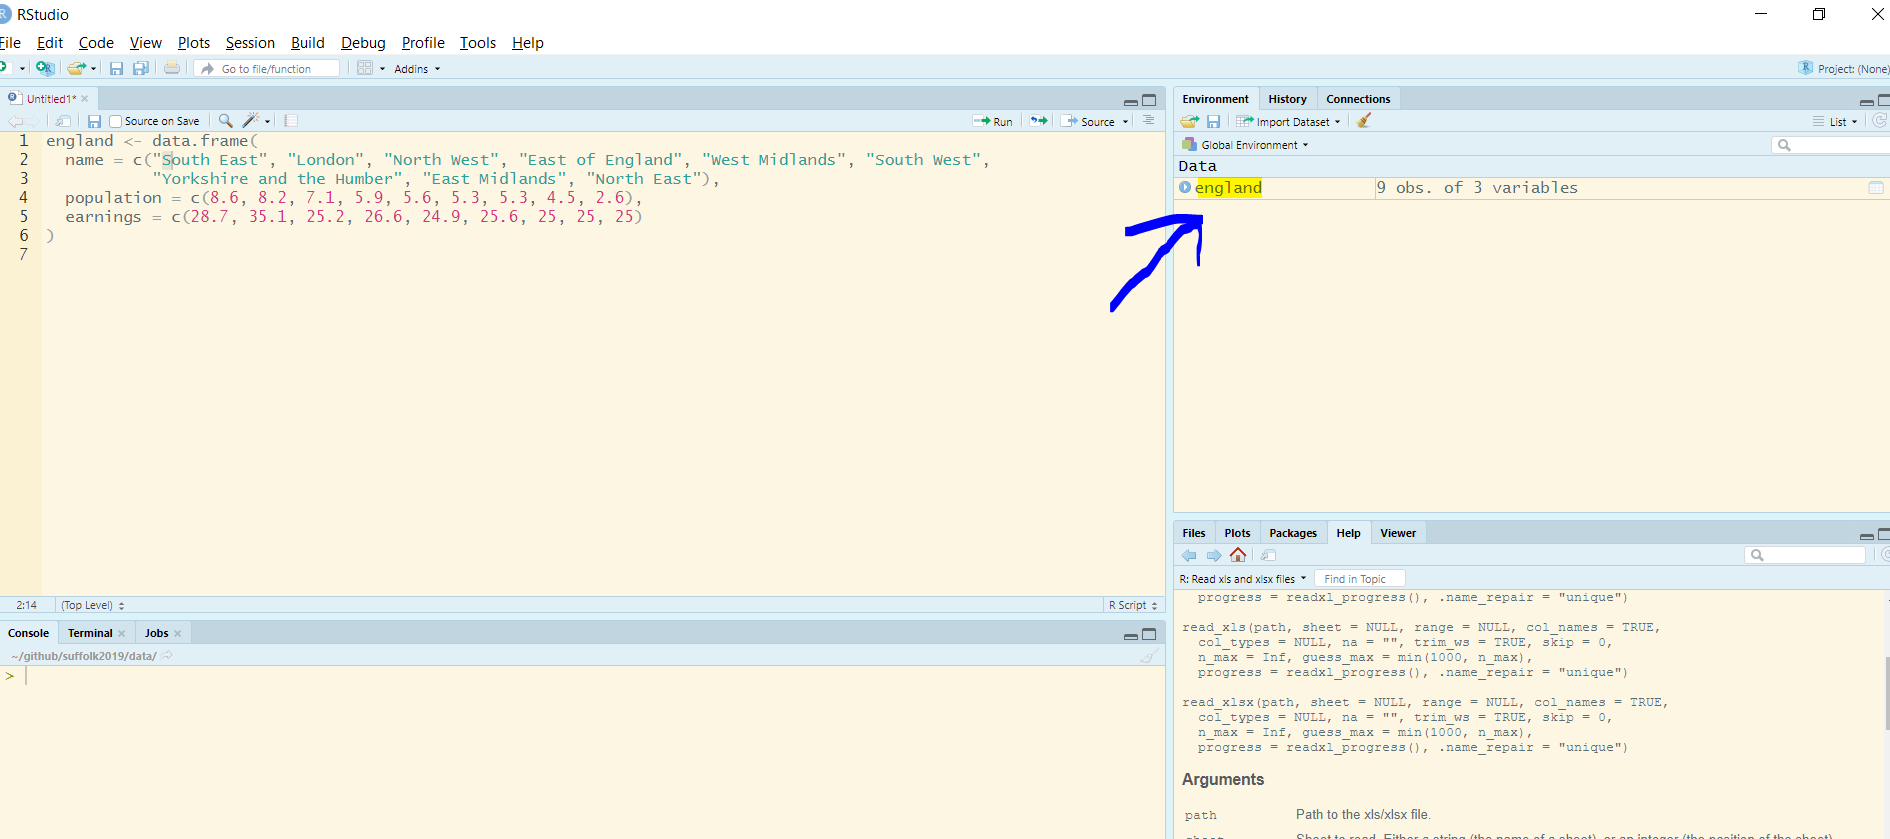
\includegraphics{./img/dataframe_in_spreadsheet_view.png}

Alternatively, you can call the object name to display the dataset in the console window. Let's do so:

\begin{Shaded}
\begin{Highlighting}[]
\NormalTok{england}
\end{Highlighting}
\end{Shaded}

\begin{verbatim}
                      name population earnings
1               South East        8.6     28.7
2                   London        8.2     35.1
3               North West        7.1     25.2
4          East of England        5.9     26.6
5            West Midlands        5.6     24.9
6               South West        5.3     25.6
7 Yorkshire and the Humber        5.3     25.0
8            East Midlands        4.5     25.0
9               North East        2.6     25.0
\end{verbatim}

Often, datasets are too long to be viewed to in the console window. It is a good idea to look at the first couple of rows of a datasets to get an overview of its contents. We use the square brackets \texttt{{[}{]}} to view the first five rows and all columns.

\begin{Shaded}
\begin{Highlighting}[]
\NormalTok{england[}\DecValTok{1}\OperatorTok{:}\DecValTok{5}\NormalTok{, ]}
\end{Highlighting}
\end{Shaded}

\begin{verbatim}
             name population earnings
1      South East        8.6     28.7
2          London        8.2     35.1
3      North West        7.1     25.2
4 East of England        5.9     26.6
5   West Midlands        5.6     24.9
\end{verbatim}

v
Columns in a dataframe have names. We will often need to know the name of a column/variable to access it. We use the \texttt{names()} function to view all variable names in a dataframe.

\begin{Shaded}
\begin{Highlighting}[]
\KeywordTok{names}\NormalTok{(england)}
\end{Highlighting}
\end{Shaded}

\begin{verbatim}
[1] "name"       "population" "earnings"  
\end{verbatim}

We can access the earnings variable in multiple ways. First, we can use the \texttt{\$} operator. We write the name of the dataset object, followed by the \texttt{\$}, followed by the variable name like so:

\begin{Shaded}
\begin{Highlighting}[]
\NormalTok{england}\OperatorTok{$}\NormalTok{earnings}
\end{Highlighting}
\end{Shaded}

\begin{verbatim}
[1] 28.7 35.1 25.2 26.6 24.9 25.6 25.0 25.0 25.0
\end{verbatim}

We can also use the square brackets to access the earnings column.

\begin{Shaded}
\begin{Highlighting}[]
\NormalTok{england[, }\StringTok{"earnings"}\NormalTok{ ]}
\end{Highlighting}
\end{Shaded}

\begin{verbatim}
[1] 28.7 35.1 25.2 26.6 24.9 25.6 25.0 25.0 25.0
\end{verbatim}

The square brackets are sometimes preferred because we could access multiple columns at once like so:

\begin{Shaded}
\begin{Highlighting}[]
\NormalTok{england[, }\KeywordTok{c}\NormalTok{(}\StringTok{"name"}\NormalTok{, }\StringTok{"earnings"}\NormalTok{) ]}
\end{Highlighting}
\end{Shaded}

\begin{verbatim}
                      name earnings
1               South East     28.7
2                   London     35.1
3               North West     25.2
4          East of England     26.6
5            West Midlands     24.9
6               South West     25.6
7 Yorkshire and the Humber     25.0
8            East Midlands     25.0
9               North East     25.0
\end{verbatim}

Variables come in different types such as numbers, text, logical (true/false). We need to know the type of a variable because the type affects statistical analysis. We use the \texttt{str()} function to check the type of each variable in our dataset.

\begin{Shaded}
\begin{Highlighting}[]
\KeywordTok{str}\NormalTok{(england)}
\end{Highlighting}
\end{Shaded}

\begin{verbatim}
'data.frame':   9 obs. of  3 variables:
 $ name      : Factor w/ 9 levels "East Midlands",..: 6 3 5 2 8 7 9 1 4
 $ population: num  8.6 8.2 7.1 5.9 5.6 5.3 5.3 4.5 2.6
 $ earnings  : num  28.7 35.1 25.2 26.6 24.9 25.6 25 25 25
\end{verbatim}

The first variable in our dataset is a factor variable. Factors are categorical variables. Categories are mutually exclusive but they do not imply an ordering. For instance, ``East of England'' is not more or less than ``West Midlands''. The variables population and earnings are both numeric variables.

\begin{Shaded}
\begin{Highlighting}[]
\KeywordTok{str}\NormalTok{(england)}
\end{Highlighting}
\end{Shaded}

\begin{verbatim}
'data.frame':   9 obs. of  3 variables:
 $ name      : Factor w/ 9 levels "East Midlands",..: 6 3 5 2 8 7 9 1 4
 $ population: num  8.6 8.2 7.1 5.9 5.6 5.3 5.3 4.5 2.6
 $ earnings  : num  28.7 35.1 25.2 26.6 24.9 25.6 25 25 25
\end{verbatim}

\hypertarget{amending-data-frames}{%
\subsubsection{Amending data frames}\label{amending-data-frames}}

Amending data sets usually involves adding rows or columns or removing rows or columns. We start by adding a new variable to our dataset which contains the percent of the population on income support.

To create a new variable we simply assign a new vector to the dataframe object like so:

\begin{Shaded}
\begin{Highlighting}[]
\NormalTok{england}\OperatorTok{$}\NormalTok{pct_on_support <-}\StringTok{ }\KeywordTok{c}\NormalTok{(}\DecValTok{3}\NormalTok{, }\FloatTok{5.3}\NormalTok{, }\FloatTok{5.3}\NormalTok{, }\FloatTok{3.5}\NormalTok{, }\FloatTok{5.1}\NormalTok{, }\FloatTok{3.3}\NormalTok{, }\FloatTok{5.2}\NormalTok{, }\FloatTok{4.2}\NormalTok{, }\FloatTok{6.1}\NormalTok{)}
\end{Highlighting}
\end{Shaded}

We call the dataframe object to view our changes.

\begin{Shaded}
\begin{Highlighting}[]
\NormalTok{england}
\end{Highlighting}
\end{Shaded}

\begin{verbatim}
                      name population earnings pct_on_support
1               South East        8.6     28.7            3.0
2                   London        8.2     35.1            5.3
3               North West        7.1     25.2            5.3
4          East of England        5.9     26.6            3.5
5            West Midlands        5.6     24.9            5.1
6               South West        5.3     25.6            3.3
7 Yorkshire and the Humber        5.3     25.0            5.2
8            East Midlands        4.5     25.0            4.2
9               North East        2.6     25.0            6.1
\end{verbatim}

We can delete the variable we just created by assigning \texttt{NULL} to it.

\begin{Shaded}
\begin{Highlighting}[]
\NormalTok{england}\OperatorTok{$}\NormalTok{pct_on_support <-}\StringTok{ }\OtherTok{NULL}
\end{Highlighting}
\end{Shaded}

Let's view our most recent changes.

\begin{Shaded}
\begin{Highlighting}[]
\NormalTok{england}
\end{Highlighting}
\end{Shaded}

\begin{verbatim}
                      name population earnings
1               South East        8.6     28.7
2                   London        8.2     35.1
3               North West        7.1     25.2
4          East of England        5.9     26.6
5            West Midlands        5.6     24.9
6               South West        5.3     25.6
7 Yorkshire and the Humber        5.3     25.0
8            East Midlands        4.5     25.0
9               North East        2.6     25.0
\end{verbatim}

Adding a new row to a dataset means adding an observation. Let's add Brittany to our dataset. We need to fill in a value for each variable. If, we do not know a value, we declare it as missing. Missings are \texttt{NA} for numeric variables and \texttt{""} for character variables. We use the \texttt{rbind()} function (row bind) to add a row to our dataset.

\begin{Shaded}
\begin{Highlighting}[]
\NormalTok{england <-}\StringTok{ }\KeywordTok{rbind}\NormalTok{(england,  }\KeywordTok{c}\NormalTok{(}\StringTok{"Brittany"}\NormalTok{, }\FloatTok{4.5}\NormalTok{, }\OtherTok{NA}\NormalTok{) )}
\end{Highlighting}
\end{Shaded}

\begin{verbatim}
Warning in `[<-.factor`(`*tmp*`, ri, value = "Brittany"): invalid factor
level, NA generated
\end{verbatim}

Let's examine our dataframe.

\begin{Shaded}
\begin{Highlighting}[]
\NormalTok{england}
\end{Highlighting}
\end{Shaded}

\begin{verbatim}
                       name population earnings
1                South East        8.6     28.7
2                    London        8.2     35.1
3                North West        7.1     25.2
4           East of England        5.9     26.6
5             West Midlands        5.6     24.9
6                South West        5.3     25.6
7  Yorkshire and the Humber        5.3       25
8             East Midlands        4.5       25
9                North East        2.6       25
10                     <NA>        4.5     <NA>
\end{verbatim}

We were not allowed to enter ``Brittany'' as a value for the name variable. This is because the variable is a factor. While it is possible to add new levels to a factor (categories such as ``Midlands'' are called levels), it involves a bit more advanced programming. We will solve this problem later in the type coercion section.

\hypertarget{saving-data-frames}{%
\subsubsection{Saving data frames}\label{saving-data-frames}}

Datasets can be exported in many different file formats. We recommend exporting files as ``.csv'' files because csv is a very common file type. Such files can be handled by all statistical packages including Microsoft's Excel. We need to provide five arguments.

\begin{longtable}[]{@{}ll@{}}
\toprule
Argument & Description\tabularnewline
\midrule
\endhead
x & The name of the object\tabularnewline
file & The file name\tabularnewline
sep & The symbol that separates columns\tabularnewline
col.names & = TRUE saves the variable names (recommended)\tabularnewline
row.names & = FALSE omits the row names (recommended)\tabularnewline
\bottomrule
\end{longtable}

\begin{Shaded}
\begin{Highlighting}[]
\KeywordTok{write.table}\NormalTok{(}\DataTypeTok{x =}\NormalTok{ england, }\DataTypeTok{file =} \StringTok{"england.csv"}\NormalTok{, }\DataTypeTok{sep =} \StringTok{","}\NormalTok{, }\DataTypeTok{col.names =} \OtherTok{TRUE}\NormalTok{, }\DataTypeTok{row.names =} \OtherTok{FALSE}\NormalTok{)}
\end{Highlighting}
\end{Shaded}

\hypertarget{type-coercion}{%
\section{Type coercion}\label{type-coercion}}

\hypertarget{seminar-3}{%
\subsection{Seminar}\label{seminar-3}}

We often need to change the type of a variable. This can be necessary to clean data or because we add a new level to a factor like in the previous section on amending data frames. We begin by loading the england dataset that we created previously.

\begin{Shaded}
\begin{Highlighting}[]
\NormalTok{england <-}\StringTok{ }\KeywordTok{read.csv}\NormalTok{(}\DataTypeTok{file =} \StringTok{"england.csv"}\NormalTok{, }\DataTypeTok{sep =} \StringTok{","}\NormalTok{, }\DataTypeTok{header =} \OtherTok{TRUE}\NormalTok{)}
\end{Highlighting}
\end{Shaded}

Recall that we could not add ``Brittany'' as a name to our variable. This was because the variable name is stored as a factor and ``Brittany'' was a new category. The easiest way to add the name ``Brittany'' is to convert the name variable into a character variable.

\hypertarget{coerce-a-factor-to-character}{%
\subsubsection{Coerce a factor to character}\label{coerce-a-factor-to-character}}

Let's check our england dataset's variable types.
.

\begin{Shaded}
\begin{Highlighting}[]
\KeywordTok{str}\NormalTok{(england)}
\end{Highlighting}
\end{Shaded}

\begin{verbatim}
'data.frame':   10 obs. of  3 variables:
 $ name      : Factor w/ 9 levels "East Midlands",..: 6 3 5 2 8 7 9 1 4 NA
 $ population: num  8.6 8.2 7.1 5.9 5.6 5.3 5.3 4.5 2.6 4.5
 $ earnings  : num  28.7 35.1 25.2 26.6 24.9 25.6 25 25 25 NA
\end{verbatim}

The variable ``name'' is a factor variable and needs to be converted to a character variable. We coerce the variable into a different type using the \texttt{as.character()} function.

\begin{Shaded}
\begin{Highlighting}[]
\NormalTok{england}\OperatorTok{$}\NormalTok{name <-}\StringTok{ }\KeywordTok{as.character}\NormalTok{(england}\OperatorTok{$}\NormalTok{name)}
\end{Highlighting}
\end{Shaded}

Let's inspect the variable types of our dataset again:

\begin{Shaded}
\begin{Highlighting}[]
\KeywordTok{str}\NormalTok{(england)}
\end{Highlighting}
\end{Shaded}

\begin{verbatim}
'data.frame':   10 obs. of  3 variables:
 $ name      : chr  "South East" "London" "North West" "East of England" ...
 $ population: num  8.6 8.2 7.1 5.9 5.6 5.3 5.3 4.5 2.6 4.5
 $ earnings  : num  28.7 35.1 25.2 26.6 24.9 25.6 25 25 25 NA
\end{verbatim}

The variable name is now a character variable. We now change the last value of the name variable into Brittany.

\begin{Shaded}
\begin{Highlighting}[]
\NormalTok{england}\OperatorTok{$}\NormalTok{name[ }\KeywordTok{length}\NormalTok{(england}\OperatorTok{$}\NormalTok{name) ] <-}\StringTok{ "Brittany"}
\end{Highlighting}
\end{Shaded}

Let's inspect our change.

\begin{Shaded}
\begin{Highlighting}[]
\NormalTok{england}
\end{Highlighting}
\end{Shaded}

\begin{verbatim}
                       name population earnings
1                South East        8.6     28.7
2                    London        8.2     35.1
3                North West        7.1     25.2
4           East of England        5.9     26.6
5             West Midlands        5.6     24.9
6                South West        5.3     25.6
7  Yorkshire and the Humber        5.3     25.0
8             East Midlands        4.5     25.0
9                North East        2.6     25.0
10                 Brittany        4.5       NA
\end{verbatim}

\hypertarget{coerce-a-character-variable-into-a-factor-variable}{%
\subsubsection{Coerce a character variable into a factor variable}\label{coerce-a-character-variable-into-a-factor-variable}}

We can now easily convert the variable type back from character into a factor with the \texttt{as.factor()} function like so:

\begin{Shaded}
\begin{Highlighting}[]
\NormalTok{england}\OperatorTok{$}\NormalTok{name <-}\StringTok{ }\KeywordTok{as.factor}\NormalTok{(england}\OperatorTok{$}\NormalTok{name)}
\KeywordTok{str}\NormalTok{(england)}
\end{Highlighting}
\end{Shaded}

\begin{verbatim}
'data.frame':   10 obs. of  3 variables:
 $ name      : Factor w/ 10 levels "Brittany","East Midlands",..: 7 4 6 3 9 8 10 2 5 1
 $ population: num  8.6 8.2 7.1 5.9 5.6 5.3 5.3 4.5 2.6 4.5
 $ earnings  : num  28.7 35.1 25.2 26.6 24.9 25.6 25 25 25 NA
\end{verbatim}

\hypertarget{coerce-a-character-variable-into-a-numeric-variable}{%
\subsubsection{Coerce a character variable into a numeric variable}\label{coerce-a-character-variable-into-a-numeric-variable}}

In R missing vlues are called \texttt{NA} for numeric types and \texttt{""} for character types. When we use load third party data, the coding often differs. This can happen, for instance, due to data entry errors.

We simulate a data entry error by changing the population value of Brittany to a character value.

\begin{Shaded}
\begin{Highlighting}[]
\NormalTok{england}\OperatorTok{$}\NormalTok{population[ }\KeywordTok{length}\NormalTok{(england}\OperatorTok{$}\NormalTok{population) ] <-}\StringTok{ "mistake"}
\KeywordTok{str}\NormalTok{(england)}
\end{Highlighting}
\end{Shaded}

\begin{verbatim}
'data.frame':   10 obs. of  3 variables:
 $ name      : Factor w/ 10 levels "Brittany","East Midlands",..: 7 4 6 3 9 8 10 2 5 1
 $ population: chr  "8.6" "8.2" "7.1" "5.9" ...
 $ earnings  : num  28.7 35.1 25.2 26.6 24.9 25.6 25 25 25 NA
\end{verbatim}

Notice, that the variable population is now a character vector instead of a numeric vector. Whenever numbers and text are mixed, R will automatically treat the vector as a character vector.

We can convert the population variable back into a numeric variable using the \texttt{as.numeric()} function. All values that are not recognised as numbers will be changed to \texttt{NA}.

\begin{Shaded}
\begin{Highlighting}[]
\NormalTok{england}\OperatorTok{$}\NormalTok{population <-}\StringTok{ }\KeywordTok{as.numeric}\NormalTok{(england}\OperatorTok{$}\NormalTok{population)}
\end{Highlighting}
\end{Shaded}

\begin{verbatim}
Warning: NAs introduced by coercion
\end{verbatim}

\begin{Shaded}
\begin{Highlighting}[]
\KeywordTok{str}\NormalTok{(england)}
\end{Highlighting}
\end{Shaded}

\begin{verbatim}
'data.frame':   10 obs. of  3 variables:
 $ name      : Factor w/ 10 levels "Brittany","East Midlands",..: 7 4 6 3 9 8 10 2 5 1
 $ population: num  8.6 8.2 7.1 5.9 5.6 5.3 5.3 4.5 2.6 NA
 $ earnings  : num  28.7 35.1 25.2 26.6 24.9 25.6 25 25 25 NA
\end{verbatim}

\begin{Shaded}
\begin{Highlighting}[]
\NormalTok{england}
\end{Highlighting}
\end{Shaded}

\begin{verbatim}
                       name population earnings
1                South East        8.6     28.7
2                    London        8.2     35.1
3                North West        7.1     25.2
4           East of England        5.9     26.6
5             West Midlands        5.6     24.9
6                South West        5.3     25.6
7  Yorkshire and the Humber        5.3     25.0
8             East Midlands        4.5     25.0
9                North East        2.6     25.0
10                 Brittany         NA       NA
\end{verbatim}

\hypertarget{loops-and-conditions}{%
\section{Loops and conditions}\label{loops-and-conditions}}

\hypertarget{seminar-4}{%
\subsection{Seminar}\label{seminar-4}}

In this section, we introduce loops and conditional statements. Loops are generally useful, when we want to carry out the same operation over and over. Conditions are logical statements that are evaluated and if the statement is true a different operation is carried out than if the statement is false. We may, for instance, be interested in the average crime rate in our sample but only if the respondents are female. To do so, we need conditional statements.

\hypertarget{for-loops}{%
\subsubsection{For loops}\label{for-loops}}

Loops are useful when we need to carry out similar operations repeatedly. A for loop is an easy way to do this. We will create a simple ``for loop'' like so:

\begin{Shaded}
\begin{Highlighting}[]
\ControlFlowTok{for}\NormalTok{ (idx }\ControlFlowTok{in} \DecValTok{1}\OperatorTok{:}\DecValTok{7}\NormalTok{)\{}
  \KeywordTok{print}\NormalTok{( idx )}
\NormalTok{\}}
\end{Highlighting}
\end{Shaded}

\begin{verbatim}
[1] 1
[1] 2
[1] 3
[1] 4
[1] 5
[1] 6
[1] 7
\end{verbatim}

In the above code, the \texttt{for()} function initiates the loop. We loop from 1 through 7 and \texttt{idx} takes the values from 1 to 7 iteratively. We can write code within the curly braces. Here, we simply print the current loop iteration.

We can create nested loops, i.e.~loops within loops like so:

\begin{Shaded}
\begin{Highlighting}[]
\CommentTok{# first loop}
\ControlFlowTok{for}\NormalTok{ (idx }\ControlFlowTok{in} \DecValTok{1}\OperatorTok{:}\DecValTok{7}\NormalTok{)\{}
  
  \CommentTok{# second loop}
  \ControlFlowTok{for}\NormalTok{ (idx2 }\ControlFlowTok{in} \DecValTok{1}\OperatorTok{:}\StringTok{ }\DecValTok{7}\NormalTok{)\{}
    
    \ControlFlowTok{if}\NormalTok{ (idx }\OperatorTok{<}\StringTok{ }\NormalTok{idx2) }\KeywordTok{print}\NormalTok{(}\StringTok{"idx1 is smaller than idx2"}\NormalTok{)}
    \ControlFlowTok{else} \KeywordTok{print}\NormalTok{(}\StringTok{"idx1 is larger than idx2"}\NormalTok{)}
    
\NormalTok{  \} }\CommentTok{# end of second loop}
\NormalTok{\} }\CommentTok{# end of first loop}
\end{Highlighting}
\end{Shaded}

\begin{verbatim}
[1] "idx1 is larger than idx2"
[1] "idx1 is smaller than idx2"
[1] "idx1 is smaller than idx2"
[1] "idx1 is smaller than idx2"
[1] "idx1 is smaller than idx2"
[1] "idx1 is smaller than idx2"
[1] "idx1 is smaller than idx2"
[1] "idx1 is larger than idx2"
[1] "idx1 is larger than idx2"
[1] "idx1 is smaller than idx2"
[1] "idx1 is smaller than idx2"
[1] "idx1 is smaller than idx2"
[1] "idx1 is smaller than idx2"
[1] "idx1 is smaller than idx2"
[1] "idx1 is larger than idx2"
[1] "idx1 is larger than idx2"
[1] "idx1 is larger than idx2"
[1] "idx1 is smaller than idx2"
[1] "idx1 is smaller than idx2"
[1] "idx1 is smaller than idx2"
[1] "idx1 is smaller than idx2"
[1] "idx1 is larger than idx2"
[1] "idx1 is larger than idx2"
[1] "idx1 is larger than idx2"
[1] "idx1 is larger than idx2"
[1] "idx1 is smaller than idx2"
[1] "idx1 is smaller than idx2"
[1] "idx1 is smaller than idx2"
[1] "idx1 is larger than idx2"
[1] "idx1 is larger than idx2"
[1] "idx1 is larger than idx2"
[1] "idx1 is larger than idx2"
[1] "idx1 is larger than idx2"
[1] "idx1 is smaller than idx2"
[1] "idx1 is smaller than idx2"
[1] "idx1 is larger than idx2"
[1] "idx1 is larger than idx2"
[1] "idx1 is larger than idx2"
[1] "idx1 is larger than idx2"
[1] "idx1 is larger than idx2"
[1] "idx1 is larger than idx2"
[1] "idx1 is smaller than idx2"
[1] "idx1 is larger than idx2"
[1] "idx1 is larger than idx2"
[1] "idx1 is larger than idx2"
[1] "idx1 is larger than idx2"
[1] "idx1 is larger than idx2"
[1] "idx1 is larger than idx2"
[1] "idx1 is larger than idx2"
\end{verbatim}

While this is a toy example, it illustrates how we could do pairwise comparisons between observations in our dataset. We also added an if/else condition using the functions \texttt{if()} and \texttt{else}. If the if statement is TRUE the first statement is printed and if not the second statement is printed.

\hypertarget{conditions}{%
\subsubsection{Conditions}\label{conditions}}

To illustrate the use of conditions we load the non-western foreigners dataset.

\begin{Shaded}
\begin{Highlighting}[]
\NormalTok{dat1 <-}\StringTok{ }\KeywordTok{read.csv}\NormalTok{(}\StringTok{"non_western_immigrants.csv"}\NormalTok{)}
\end{Highlighting}
\end{Shaded}

\begin{longtable}[]{@{}ll@{}}
\toprule
\begin{minipage}[b]{0.11\columnwidth}\raggedright
Variable Name\strut
\end{minipage} & \begin{minipage}[b]{0.83\columnwidth}\raggedright
Description\strut
\end{minipage}\tabularnewline
\midrule
\endhead
\begin{minipage}[t]{0.11\columnwidth}\raggedright
IMMBRIT\strut
\end{minipage} & \begin{minipage}[t]{0.83\columnwidth}\raggedright
Out of every 100 people in Britain, how many do you think are immigrants from Non-western countries?\strut
\end{minipage}\tabularnewline
\begin{minipage}[t]{0.11\columnwidth}\raggedright
over.estimate\strut
\end{minipage} & \begin{minipage}[t]{0.83\columnwidth}\raggedright
1 if estimate is higher than 10.7\%.\strut
\end{minipage}\tabularnewline
\begin{minipage}[t]{0.11\columnwidth}\raggedright
RSex\strut
\end{minipage} & \begin{minipage}[t]{0.83\columnwidth}\raggedright
1 = male, 2 = female\strut
\end{minipage}\tabularnewline
\begin{minipage}[t]{0.11\columnwidth}\raggedright
RAge\strut
\end{minipage} & \begin{minipage}[t]{0.83\columnwidth}\raggedright
Age of respondent\strut
\end{minipage}\tabularnewline
\begin{minipage}[t]{0.11\columnwidth}\raggedright
Househld\strut
\end{minipage} & \begin{minipage}[t]{0.83\columnwidth}\raggedright
Number of people living in respondent's household\strut
\end{minipage}\tabularnewline
\begin{minipage}[t]{0.11\columnwidth}\raggedright
Cons, Lab, SNP, Ukip, BNP, GP, party.other\strut
\end{minipage} & \begin{minipage}[t]{0.83\columnwidth}\raggedright
Party self-identification\strut
\end{minipage}\tabularnewline
\begin{minipage}[t]{0.11\columnwidth}\raggedright
paper\strut
\end{minipage} & \begin{minipage}[t]{0.83\columnwidth}\raggedright
Do you normally read any daily morning newspaper 3+ times/week?\strut
\end{minipage}\tabularnewline
\begin{minipage}[t]{0.11\columnwidth}\raggedright
WWWhourspW\strut
\end{minipage} & \begin{minipage}[t]{0.83\columnwidth}\raggedright
How many hours WWW per week?\strut
\end{minipage}\tabularnewline
\begin{minipage}[t]{0.11\columnwidth}\raggedright
religious\strut
\end{minipage} & \begin{minipage}[t]{0.83\columnwidth}\raggedright
Do you regard yourself as belonging to any particular religion?\strut
\end{minipage}\tabularnewline
\begin{minipage}[t]{0.11\columnwidth}\raggedright
employMonths\strut
\end{minipage} & \begin{minipage}[t]{0.83\columnwidth}\raggedright
How many mnths w. present employer?\strut
\end{minipage}\tabularnewline
\begin{minipage}[t]{0.11\columnwidth}\raggedright
urban\strut
\end{minipage} & \begin{minipage}[t]{0.83\columnwidth}\raggedright
Population density, 4 categories (highest density is 4, lowest is 1)\strut
\end{minipage}\tabularnewline
\begin{minipage}[t]{0.11\columnwidth}\raggedright
health.good\strut
\end{minipage} & \begin{minipage}[t]{0.83\columnwidth}\raggedright
How is your health in general for someone of your age? (0: bad, 1: fair, 2: fairly good, 3: good)\strut
\end{minipage}\tabularnewline
\begin{minipage}[t]{0.11\columnwidth}\raggedright
HHInc\strut
\end{minipage} & \begin{minipage}[t]{0.83\columnwidth}\raggedright
Income bands for household, high number = high HH income\strut
\end{minipage}\tabularnewline
\bottomrule
\end{longtable}

The variable \texttt{over.estimate} is equal to 1 if respondents over estimate the number of non-western immigrants in Britain. We will evaluate whether women are more or less likely to over estimate. First, we use the \texttt{mean()} function to assess the overall average value.

\begin{Shaded}
\begin{Highlighting}[]
\KeywordTok{mean}\NormalTok{(dat1}\OperatorTok{$}\NormalTok{over.estimate)}
\end{Highlighting}
\end{Shaded}

\begin{verbatim}
[1] 0.7235462
\end{verbatim}

A mean of 0.72 indicates that 72\% of the 1049 respondents in the dataset over estimate the number of non-western immigrants. To assess whether the number is larger among men than women, we need conditional statements.

We first take the mean of ``over.estimate'' for men:

\begin{Shaded}
\begin{Highlighting}[]
\KeywordTok{mean}\NormalTok{( dat1}\OperatorTok{$}\NormalTok{over.estimate[ dat1}\OperatorTok{$}\NormalTok{RSex}\OperatorTok{==}\DecValTok{1}\NormalTok{ ] )}
\end{Highlighting}
\end{Shaded}

\begin{verbatim}
[1] 0.6527197
\end{verbatim}

Here, we used square brackets to subset the data. The subset that we evaluate is described by the logical statement \texttt{dat1\$RSex==1}. The \texttt{==} operator is a logical equal that is true if a condition is fulfilled and false otherwise. In this case, it is true if the variable ``RSex'' is 1 which stands for men.

Take the mean of over.estimate for women on your own.

\begin{Shaded}
\begin{Highlighting}[]
\KeywordTok{mean}\NormalTok{( dat1}\OperatorTok{$}\NormalTok{over.estimate[ dat1}\OperatorTok{$}\NormalTok{RSex}\OperatorTok{==}\StringTok{ }\DecValTok{2}\NormalTok{] )}
\end{Highlighting}
\end{Shaded}

\begin{verbatim}
[1] 0.7828371
\end{verbatim}

It turns out, that females in our sample over estimate the number of non-western immigrants more. Whether the difference in our sample is systematic, i.e.~whether it would hold in the population as well is a matter that we will return to.

Here we have taken two conditional means and compared them. Doing so is the first step towards statistical inference.

\hypertarget{the-ifelse-function}{%
\subsubsection{The ifelse() function}\label{the-ifelse-function}}

Categorical variables such as ``RSex'' are usually coded 0/1 and the variable name usually refers to the category that is 1. ``RSex'' is a bad variable name because it is not clear whehter the values 1 and 2 refer to males or females.

We will create a new variable called ``female'' that is equal to 1 if the respondent is female and 0 otherwise. We do so using the \texttt{ifelse()} function. The function first evaluates a logical condition and subsequently carries out one operation if the statement is true (yes) and another if the statement is false (no).

\begin{Shaded}
\begin{Highlighting}[]
\NormalTok{dat1}\OperatorTok{$}\NormalTok{female <-}\StringTok{ }\KeywordTok{ifelse}\NormalTok{( dat1}\OperatorTok{$}\NormalTok{RSex }\OperatorTok{==}\StringTok{ }\DecValTok{2}\NormalTok{, }\DataTypeTok{yes =} \DecValTok{1}\NormalTok{, }\DataTypeTok{no =} \DecValTok{0}\NormalTok{ )}
\end{Highlighting}
\end{Shaded}

Let's check whetehr we correctly converted the variable using the \texttt{table()} function which produces a frequency table.

\begin{Shaded}
\begin{Highlighting}[]
\KeywordTok{table}\NormalTok{(dat1}\OperatorTok{$}\NormalTok{RSex)}
\end{Highlighting}
\end{Shaded}

\begin{verbatim}

  1   2 
478 571 
\end{verbatim}

\begin{Shaded}
\begin{Highlighting}[]
\KeywordTok{table}\NormalTok{(dat1}\OperatorTok{$}\NormalTok{female)}
\end{Highlighting}
\end{Shaded}

\begin{verbatim}

  0   1 
478 571 
\end{verbatim}

\hypertarget{visualising-data}{%
\section{Visualising data}\label{visualising-data}}

\hypertarget{seminar-5}{%
\subsection{Seminar}\label{seminar-5}}

In this section, we will learn how to visualise data which is an important step towards understanding relationships better.

The non-western foreingers data is about the subjective perception of immigrants from non-western countries. The perception of immigrants from a context that is not similar to the one's own ,is often used as a proxy for racism. Whether this is a fair measure or not is debatable but let's examine the data from a survey carried out in Britain.

Let's check the codebook of our data.

\begin{tabular}{l|l}
\hline
Variable & Description\\
\hline
IMMBRIT & Out of every 100 people in Britain, how many do you think are immigrants from non-western countries?\\
\hline
over.estimate & 1 if estimate is higher than 10.7\%.\\
\hline
RSex & 1 = male, 2 = female\\
\hline
RAge & Age of respondent\\
\hline
Househld & Number of people living in respondent's household\\
\hline
party identification & 1 = Conservatives, 2 = Labour, 3 = SNP, 4 = Greens, 5 = Ukip, 6 = BNP, 7 = other\\
\hline
paper & Do you normally read any daily morning newspaper 3+ times/week?\\
\hline
WWWhourspW & How many hours WWW per week?\\
\hline
religious & Do you regard yourself as belonging to any particular religion?\\
\hline
employMonths & How many mnths w. present employer?\\
\hline
urban & Population density, 4 categories (highest density is 4, lowest is 1)\\
\hline
health.good & How is your health in general for someone of your age? (0: bad, 1: fair, 2: fairly good, 3: good)\\
\hline
HHInc & Income bands for household, high number = high HH income\\
\hline
\end{tabular}

Let's load the dataset.

\begin{Shaded}
\begin{Highlighting}[]
\NormalTok{dat1 <-}\StringTok{ }\KeywordTok{read.csv}\NormalTok{(}\StringTok{"non_western_immigrants.csv"}\NormalTok{)}
\end{Highlighting}
\end{Shaded}

We can look at the variable names in our data with the \href{http://bit.ly/R_names}{\texttt{names()}} function.

The \href{http://bit.ly/R_dim}{\texttt{dim()}} function can be used to find out the dimensions of the dataset (dimension 1 = rows, dimension 2 = columns).

\begin{Shaded}
\begin{Highlighting}[]
\KeywordTok{dim}\NormalTok{(dat1)}
\end{Highlighting}
\end{Shaded}

\begin{verbatim}
[1] 1049   13
\end{verbatim}

So, the \href{http://bit.ly/R_dim}{\texttt{dim()}} function tells us that we have data from 1049 respondents with 13 variables for each respondent.

Let's take a quick peek at the first 10 observations to see what the dataset looks like. By default the \href{http://bit.ly/R_head}{\texttt{head()}} function returns the first 6 rows, but let's tell it to return the first 10 rows instead.

\begin{Shaded}
\begin{Highlighting}[]
\KeywordTok{head}\NormalTok{(dat1, }\DataTypeTok{n =} \DecValTok{10}\NormalTok{)}
\end{Highlighting}
\end{Shaded}

\begin{verbatim}
   IMMBRIT over.estimate RSex RAge Househld paper WWWhourspW religious
1        1             0    1   50        2     0          1         0
2       50             1    2   18        3     0          4         0
3       50             1    2   60        1     0          1         0
4       15             1    2   77        2     1          2         1
5       20             1    2   67        1     0          1         1
6       30             1    1   30        4     1         14         0
7       60             1    2   56        2     0          5         1
8        7             0    1   49        1     1          8         0
9       30             1    1   40        4     0          3         1
10       2             0    1   61        3     1          0         1
   employMonths urban health.good HHInc party_self
1            72     4           1    13          2
2            72     4           2     3          7
3           456     3           3     9          7
4            72     1           3     8          7
5            72     3           3     9          7
6            72     1           2     9          7
7           180     1           2    13          3
8           156     4           2    14          7
9           264     2           2    11          3
10           72     1           3     8          1
\end{verbatim}

Finally, let's look at summary statistics of our dataset.

\begin{Shaded}
\begin{Highlighting}[]
\KeywordTok{summary}\NormalTok{(dat1)}
\end{Highlighting}
\end{Shaded}

\begin{verbatim}
    IMMBRIT       over.estimate         RSex            RAge      
 Min.   :  0.00   Min.   :0.0000   Min.   :1.000   Min.   :17.00  
 1st Qu.: 10.00   1st Qu.:0.0000   1st Qu.:1.000   1st Qu.:36.00  
 Median : 25.00   Median :1.0000   Median :2.000   Median :49.00  
 Mean   : 29.03   Mean   :0.7235   Mean   :1.544   Mean   :49.75  
 3rd Qu.: 40.00   3rd Qu.:1.0000   3rd Qu.:2.000   3rd Qu.:62.00  
 Max.   :100.00   Max.   :1.0000   Max.   :2.000   Max.   :99.00  
    Househld         paper          WWWhourspW        religious     
 Min.   :1.000   Min.   :0.0000   Min.   :  0.000   Min.   :0.0000  
 1st Qu.:1.000   1st Qu.:0.0000   1st Qu.:  0.000   1st Qu.:0.0000  
 Median :2.000   Median :0.0000   Median :  2.000   Median :0.0000  
 Mean   :2.392   Mean   :0.4538   Mean   :  5.251   Mean   :0.4929  
 3rd Qu.:3.000   3rd Qu.:1.0000   3rd Qu.:  7.000   3rd Qu.:1.0000  
 Max.   :8.000   Max.   :1.0000   Max.   :100.000   Max.   :1.0000  
  employMonths        urban        health.good        HHInc       
 Min.   :  1.00   Min.   :1.000   Min.   :0.000   Min.   : 1.000  
 1st Qu.: 72.00   1st Qu.:2.000   1st Qu.:2.000   1st Qu.: 6.000  
 Median : 72.00   Median :3.000   Median :2.000   Median : 9.000  
 Mean   : 86.56   Mean   :2.568   Mean   :2.044   Mean   : 9.586  
 3rd Qu.: 72.00   3rd Qu.:3.000   3rd Qu.:3.000   3rd Qu.:13.000  
 Max.   :600.00   Max.   :4.000   Max.   :3.000   Max.   :17.000  
   party_self   
 Min.   :1.000  
 1st Qu.:1.000  
 Median :2.000  
 Mean   :3.825  
 3rd Qu.:7.000  
 Max.   :7.000  
\end{verbatim}

\hypertarget{plots}{%
\subsubsection{Plots}\label{plots}}

We can visualize the data with the help of a boxplot, so let's see how the perception of the number of immigrants is distributed.

\begin{Shaded}
\begin{Highlighting}[]
\CommentTok{# how good are we at guessing immigration}
\KeywordTok{boxplot}\NormalTok{(}
\NormalTok{  dat1}\OperatorTok{$}\NormalTok{IMMBRIT, }
  \DataTypeTok{main =} \StringTok{"Perception of Immigration from Non-Western Countries"}\NormalTok{,}
  \DataTypeTok{ylab =} \StringTok{"Subjective number of immigrants per 100 British"}\NormalTok{, }
  \DataTypeTok{frame.plot =} \OtherTok{FALSE}\NormalTok{, }\DataTypeTok{col =} \StringTok{"darkgray"}
\NormalTok{  )}
\end{Highlighting}
\end{Shaded}

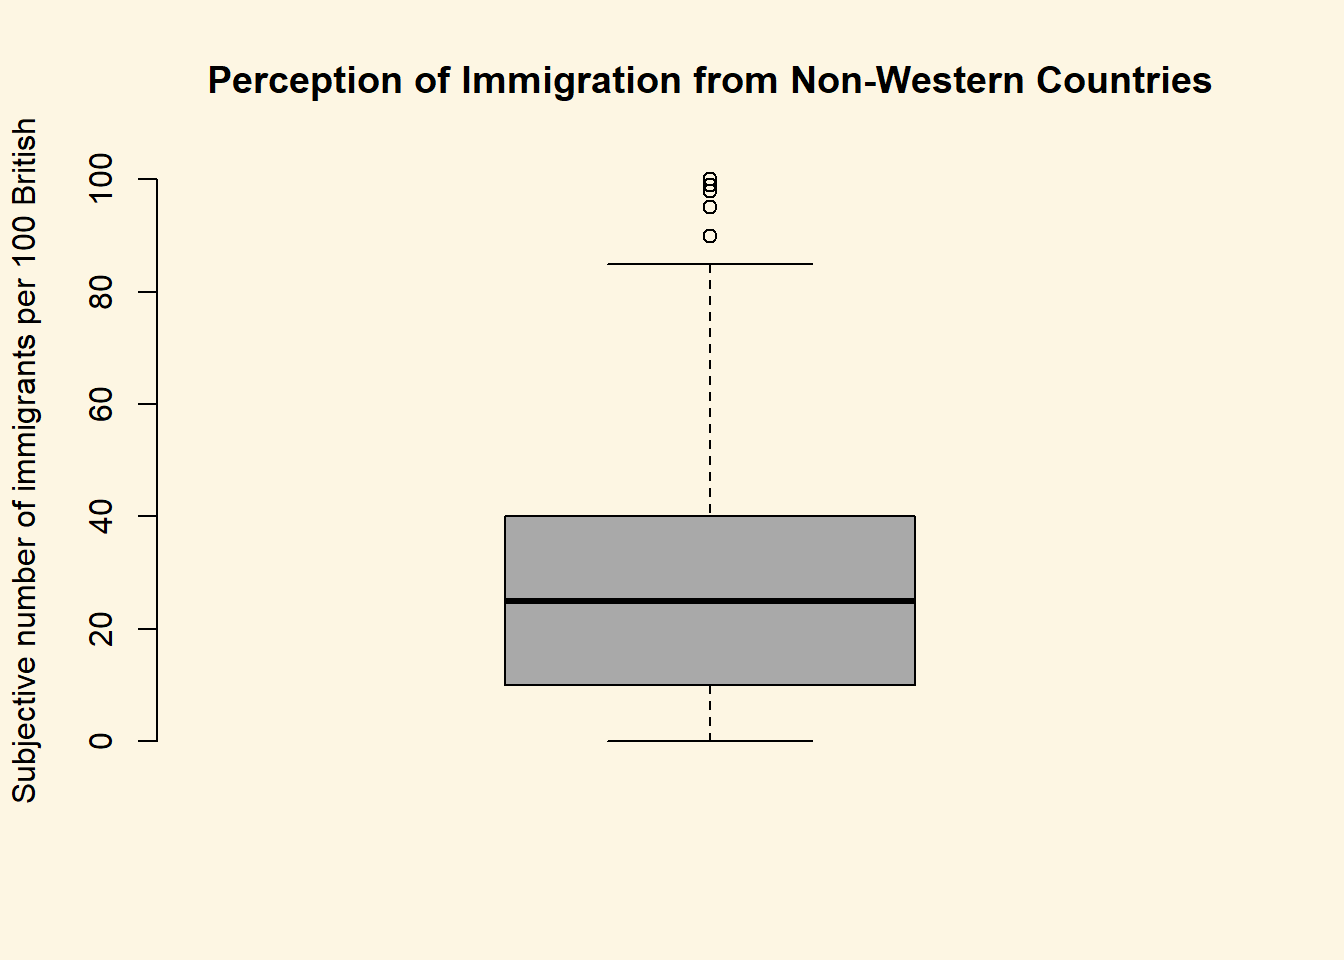
\includegraphics{suffolk2019_files/figure-latex/unnamed-chunk-87-1.pdf}

Notice how the lower whisker is much shorter than the upper one. The distribution is right skewed. The right tail (higher values) is a lot longer. We can see this beter using a density plot. We combine R's \texttt{denisty()} function with the \texttt{plot()} function.

\begin{Shaded}
\begin{Highlighting}[]
\KeywordTok{plot}\NormalTok{(}
  \KeywordTok{density}\NormalTok{(dat1}\OperatorTok{$}\NormalTok{IMMBRIT),}
  \DataTypeTok{bty =} \StringTok{"n"}\NormalTok{,}
  \DataTypeTok{main =} \StringTok{"Perception of Immigration from Non-Western Countries"}\NormalTok{,}
  \DataTypeTok{xlab =} \StringTok{"Subjective number of immigrants per 100 British"}
\NormalTok{  )}
\end{Highlighting}
\end{Shaded}

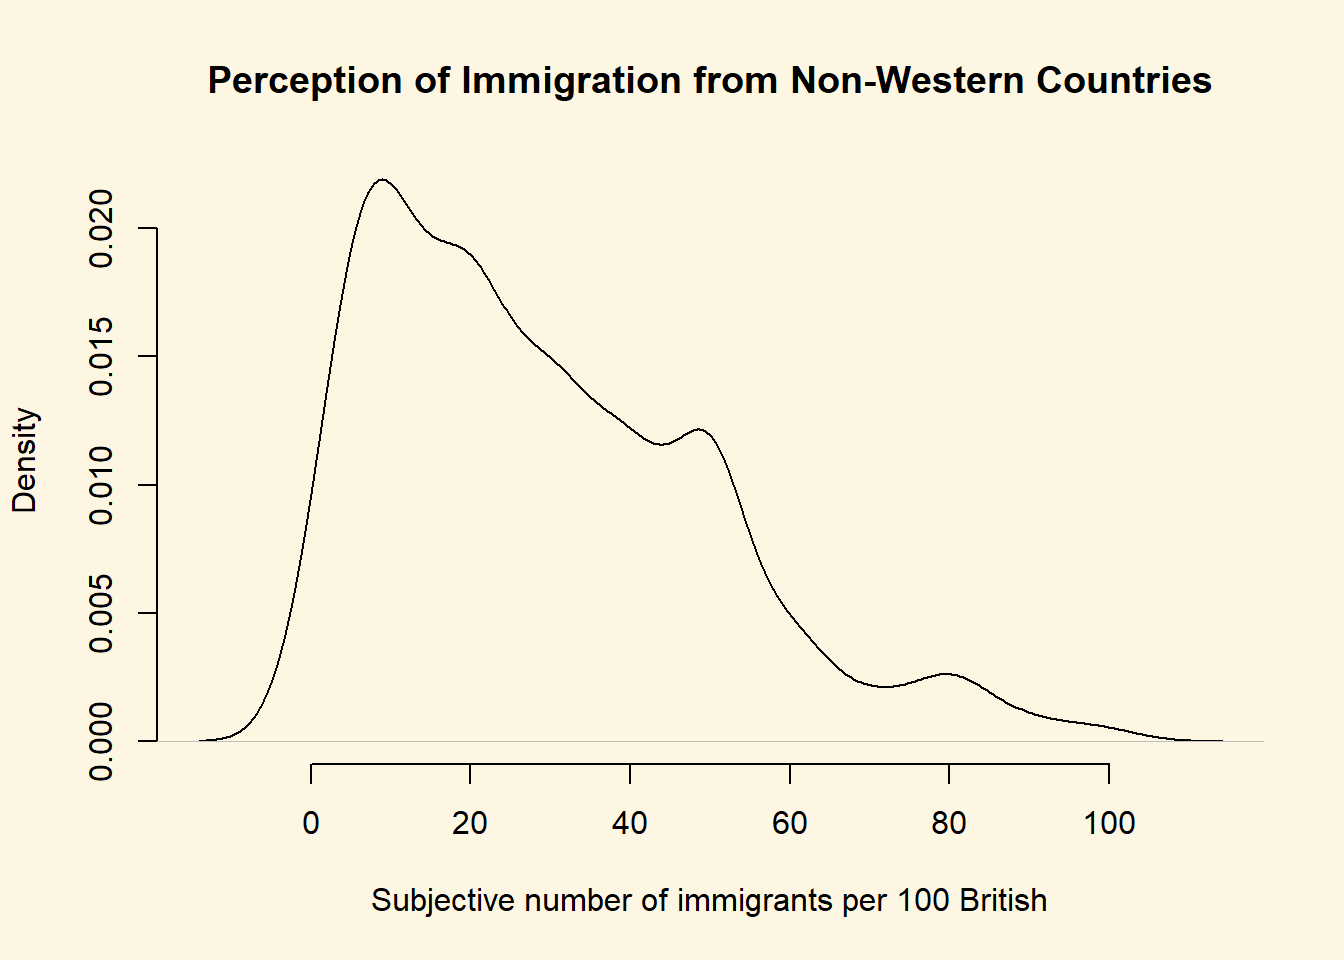
\includegraphics{suffolk2019_files/figure-latex/unnamed-chunk-88-1.pdf}

We can also plot histograms using the \texttt{hist()} function.

\begin{Shaded}
\begin{Highlighting}[]
\CommentTok{# histogram}
\KeywordTok{hist}\NormalTok{( dat1}\OperatorTok{$}\NormalTok{employMonths, }\DataTypeTok{main =} \StringTok{"histogram"}\NormalTok{)}
\end{Highlighting}
\end{Shaded}

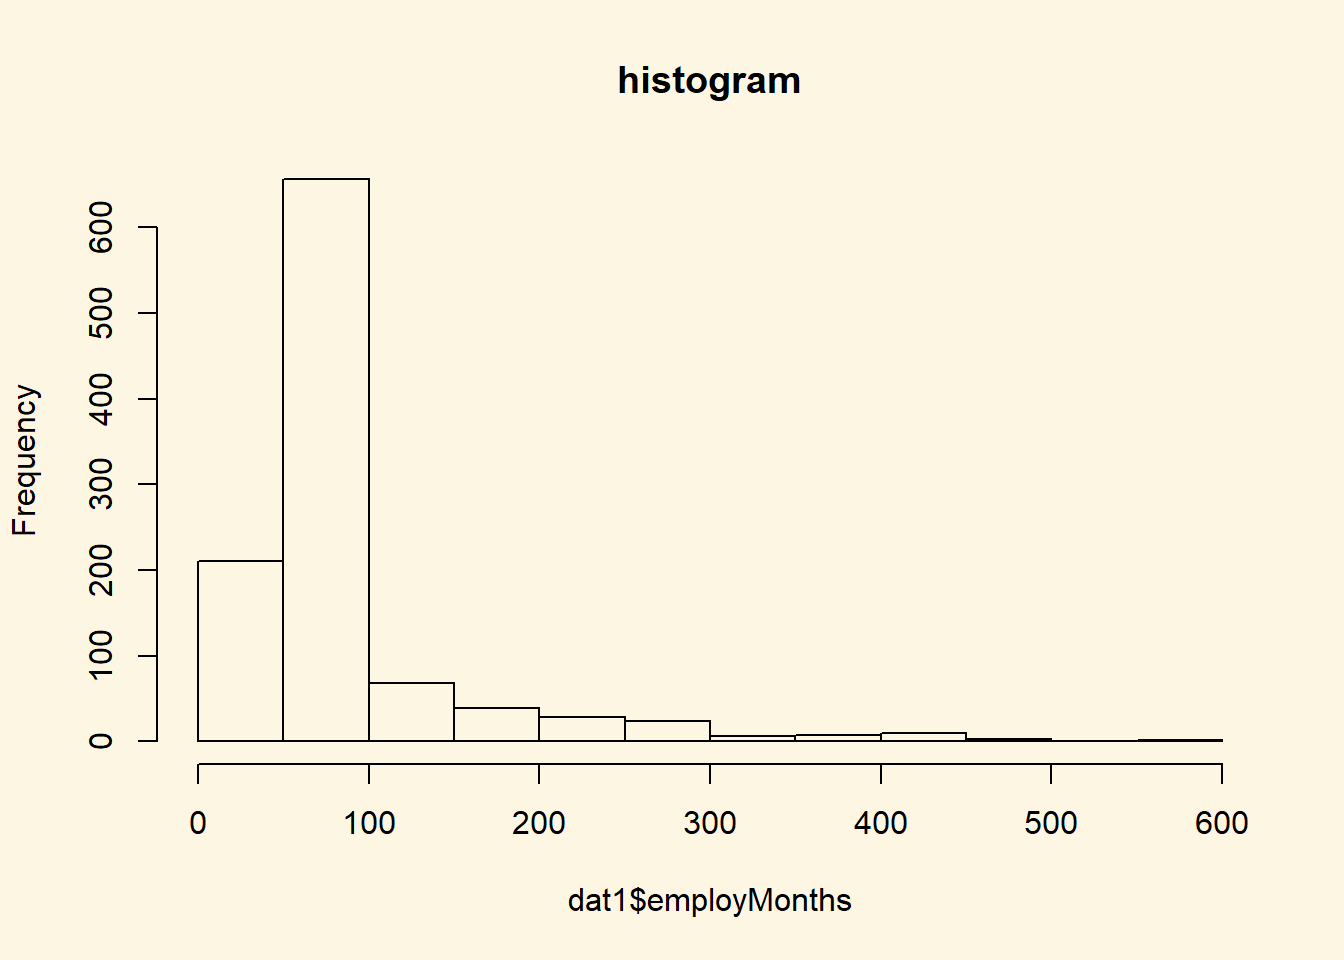
\includegraphics{suffolk2019_files/figure-latex/unnamed-chunk-89-1.pdf}

It is plausible that perception of immigration from Non-Western countries is related to party affiliation. In our dataset, we have a some party affiliation dummies (binary variables). We can use square brackets to subset our data such that we produce a boxplot only for members of the Conservative Party. We first create the binary variables \emph{Cons} and \emph{Lab} for (Conservatives and Labour respectively) using the \texttt{ifelse()} function.

\begin{Shaded}
\begin{Highlighting}[]
\NormalTok{dat1}\OperatorTok{$}\NormalTok{Cons <-}\StringTok{ }\KeywordTok{ifelse}\NormalTok{(dat1}\OperatorTok{$}\NormalTok{party_self }\OperatorTok{==}\StringTok{ }\DecValTok{1}\NormalTok{, }\DataTypeTok{yes =} \DecValTok{1}\NormalTok{, }\DataTypeTok{no =} \DecValTok{0}\NormalTok{)}
\NormalTok{dat1}\OperatorTok{$}\NormalTok{Lab <-}\StringTok{ }\KeywordTok{ifelse}\NormalTok{(dat1}\OperatorTok{$}\NormalTok{party_self }\OperatorTok{==}\StringTok{ }\DecValTok{2}\NormalTok{, }\DataTypeTok{yes =} \DecValTok{1}\NormalTok{, }\DataTypeTok{no =} \DecValTok{0}\NormalTok{)}
\end{Highlighting}
\end{Shaded}

We have a look at the variable \emph{Cons} using the \texttt{table()} function first.

\begin{Shaded}
\begin{Highlighting}[]
\KeywordTok{table}\NormalTok{(dat1}\OperatorTok{$}\NormalTok{Cons)}
\end{Highlighting}
\end{Shaded}

\begin{verbatim}

  0   1 
765 284 
\end{verbatim}

In our data, 284 respondents associate with the Conservative party and 765 do not. We create a boxplot of \emph{IMMBRIT} but only for members of the Conservative Party. We do so by using the square brackets to subset our data.

\begin{Shaded}
\begin{Highlighting}[]
\CommentTok{# boxplot of immbrit for those observations where Cons is 1}
\KeywordTok{boxplot}\NormalTok{(}
\NormalTok{  dat1}\OperatorTok{$}\NormalTok{IMMBRIT[dat1}\OperatorTok{$}\NormalTok{Cons}\OperatorTok{==}\DecValTok{1}\NormalTok{],}
  \DataTypeTok{frame.plot =} \OtherTok{FALSE}\NormalTok{,}
  \DataTypeTok{xlab =} \StringTok{"Conservatives"}\NormalTok{,}
  \DataTypeTok{col =} \StringTok{"blue"}
\NormalTok{  )}
\end{Highlighting}
\end{Shaded}

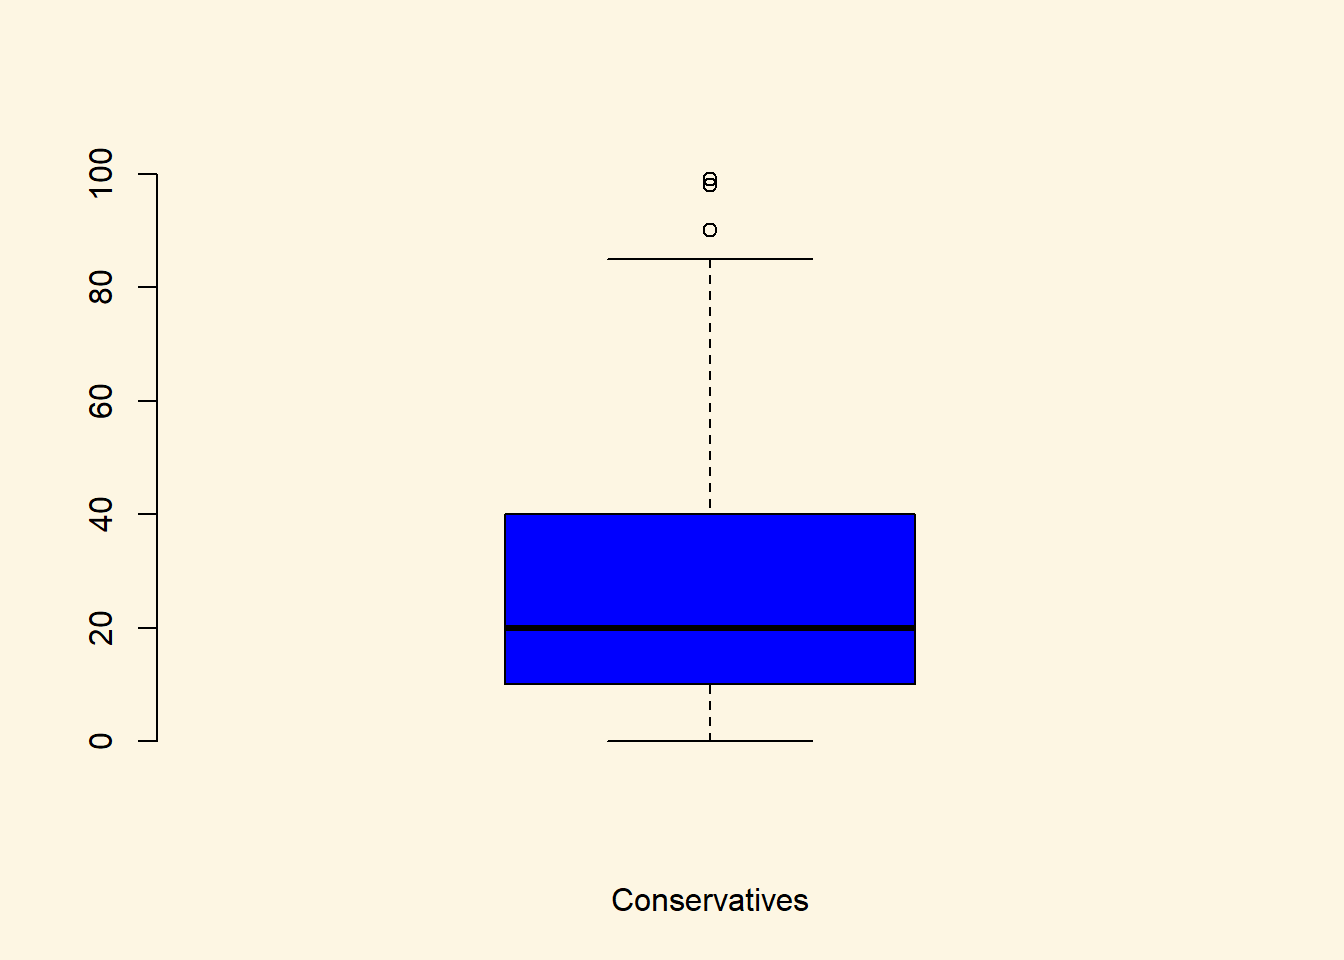
\includegraphics{suffolk2019_files/figure-latex/unnamed-chunk-92-1.pdf}

We would now like to compare the distribution of the perception fo Conservatives to the distribution among Labour respondents. We can subset the data just like we did for the Conservative Party. In addtion, we want to plot the two plots next to each other, i.e., they should be in the same plot. We can achieve this with the \texttt{par()} function and the \texttt{mfrow} argument. This will spilt the plot window into rows and columns. We want 2 columns to plot 2 boxplots next to each other.

\begin{Shaded}
\begin{Highlighting}[]
\CommentTok{# split plot window into 1 row and 2 columns}
\KeywordTok{par}\NormalTok{(}\DataTypeTok{mfrow =} \KeywordTok{c}\NormalTok{(}\DecValTok{1}\NormalTok{,}\DecValTok{2}\NormalTok{))}

\CommentTok{# plot 1}
\KeywordTok{boxplot}\NormalTok{(}
\NormalTok{  dat1}\OperatorTok{$}\NormalTok{IMMBRIT[dat1}\OperatorTok{$}\NormalTok{Cons}\OperatorTok{==}\DecValTok{1}\NormalTok{],}
  \DataTypeTok{frame.plot =} \OtherTok{FALSE}\NormalTok{,}
  \DataTypeTok{xlab =} \StringTok{"Conservatives"}\NormalTok{,}
  \DataTypeTok{col =} \StringTok{"blue"}
\NormalTok{  )}

\CommentTok{# plot 2}
\KeywordTok{boxplot}\NormalTok{(}
\NormalTok{  dat1}\OperatorTok{$}\NormalTok{IMMBRIT[dat1}\OperatorTok{$}\NormalTok{Lab}\OperatorTok{==}\DecValTok{1}\NormalTok{],}
  \DataTypeTok{frame.plot =} \OtherTok{FALSE}\NormalTok{,}
  \DataTypeTok{xlab =} \StringTok{"Labour"}\NormalTok{,}
  \DataTypeTok{col =} \StringTok{"red"}
\NormalTok{  )}
\end{Highlighting}
\end{Shaded}

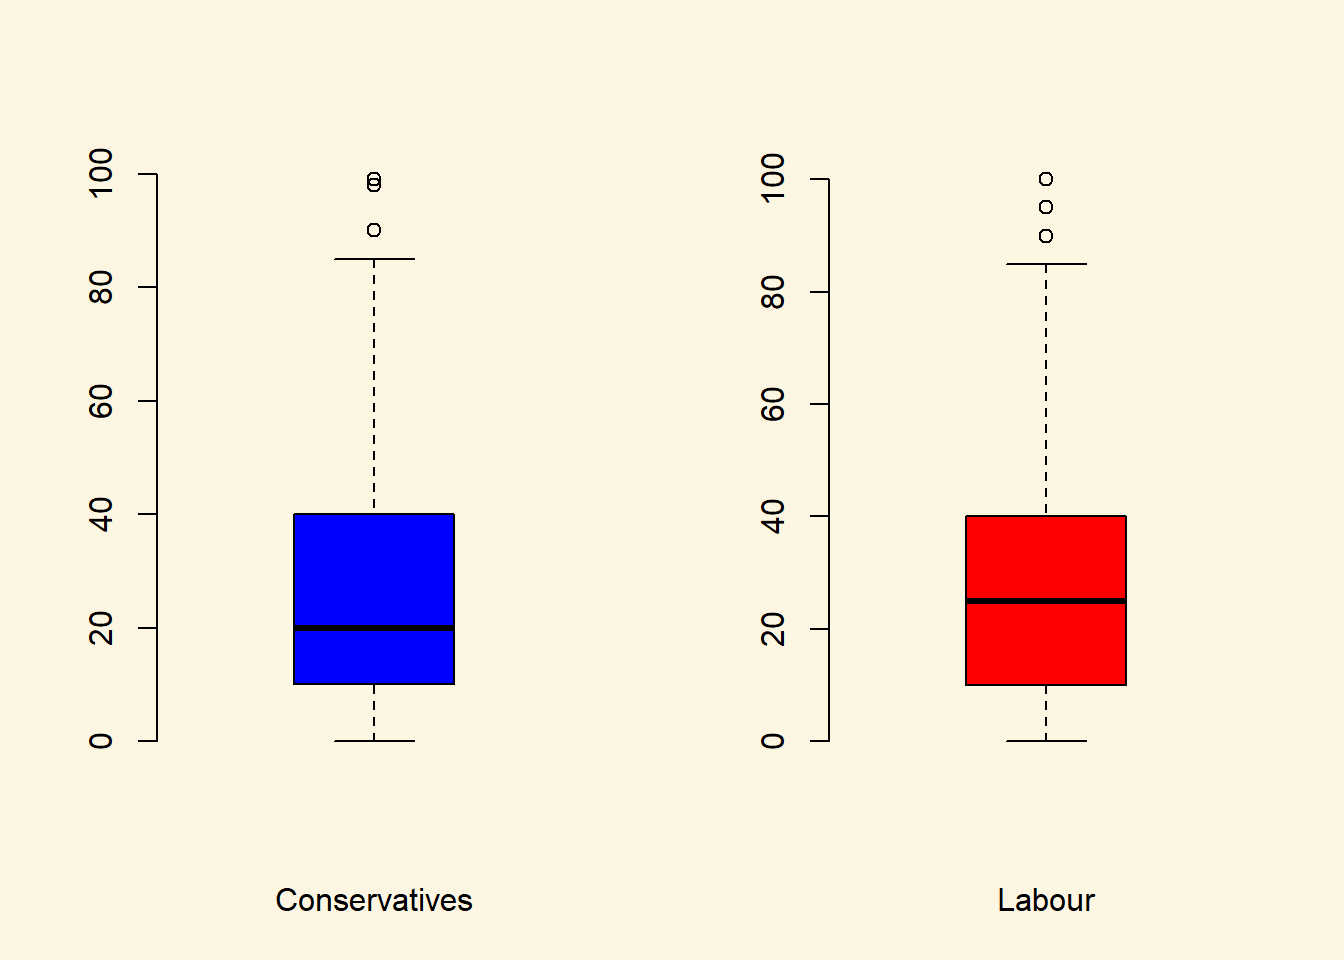
\includegraphics{suffolk2019_files/figure-latex/unnamed-chunk-93-1.pdf}

It is very hard to spot differences. The distributions are similar. The median for Labour respondents is larger which mean that the central Labour respondent over-estimates immigration more than the central Conservative respondent.

You can play around with the non-western foreigners data on your own time. We now turn to a dataset that is integrated in R already. It is called \texttt{longley}. Use the \texttt{help()} function to see what this dataset is about.

\begin{Shaded}
\begin{Highlighting}[]
\KeywordTok{help}\NormalTok{(longley)}
\end{Highlighting}
\end{Shaded}

Let's create a scatterplot with the \texttt{Year} variable on the x-axis and \texttt{Employed} on the y-axis.

\begin{Shaded}
\begin{Highlighting}[]
\KeywordTok{plot}\NormalTok{(}\DataTypeTok{x =}\NormalTok{ longley}\OperatorTok{$}\NormalTok{Year, }\CommentTok{# x-axis variable}
     \DataTypeTok{y =}\NormalTok{ longley}\OperatorTok{$}\NormalTok{Employed, }\CommentTok{# y-axis variable}
     \DataTypeTok{bty =} \StringTok{"n"} \CommentTok{# no box around the plot}
\NormalTok{     )}
\end{Highlighting}
\end{Shaded}

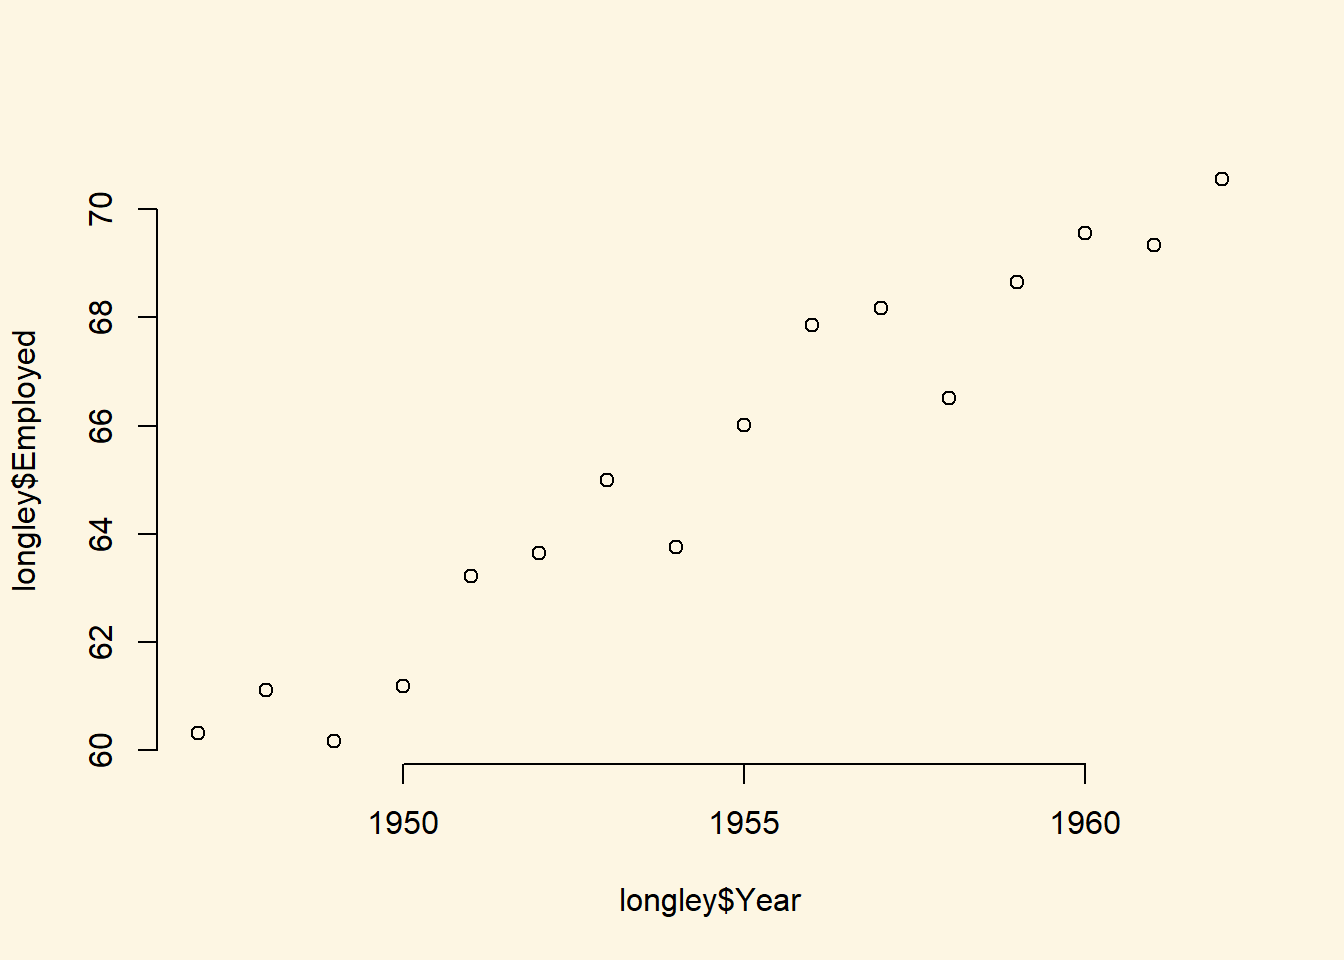
\includegraphics{suffolk2019_files/figure-latex/unnamed-chunk-96-1.pdf}

To create a line plot instead, we use the same function with one additional argument \texttt{type\ =\ "l"}.

\begin{Shaded}
\begin{Highlighting}[]
\KeywordTok{plot}\NormalTok{(longley}\OperatorTok{$}\NormalTok{Year, longley}\OperatorTok{$}\NormalTok{Employed, }\DataTypeTok{type =} \StringTok{"l"}\NormalTok{)}
\end{Highlighting}
\end{Shaded}

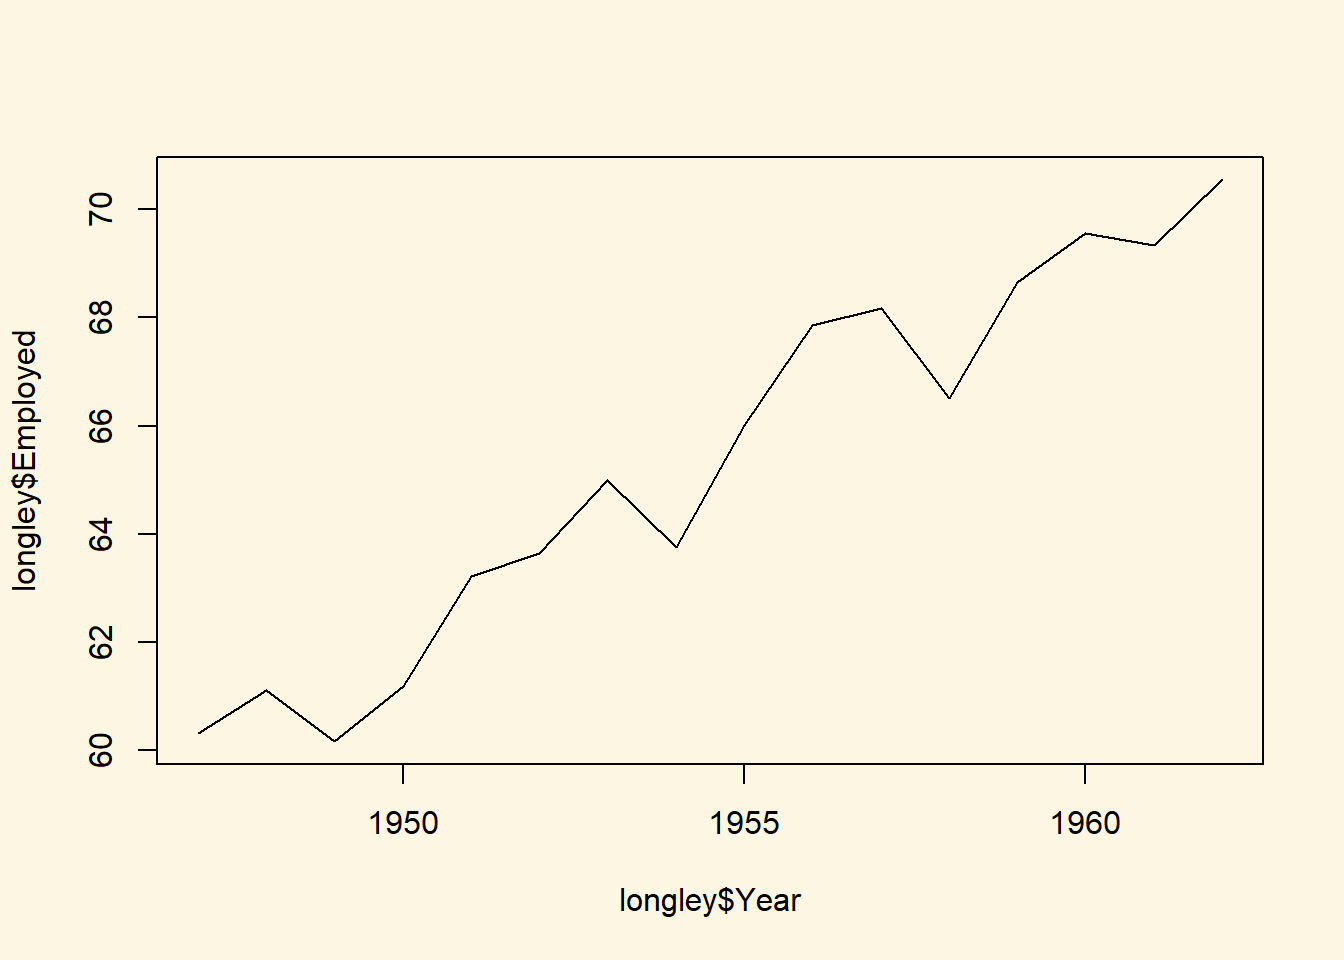
\includegraphics{suffolk2019_files/figure-latex/unnamed-chunk-97-1.pdf}

Create a plot that includes both points and lines.

\begin{Shaded}
\begin{Highlighting}[]
\KeywordTok{plot}\NormalTok{(longley}\OperatorTok{$}\NormalTok{Year, longley}\OperatorTok{$}\NormalTok{Employed, }\DataTypeTok{type =} \StringTok{"b"}\NormalTok{)}
\end{Highlighting}
\end{Shaded}

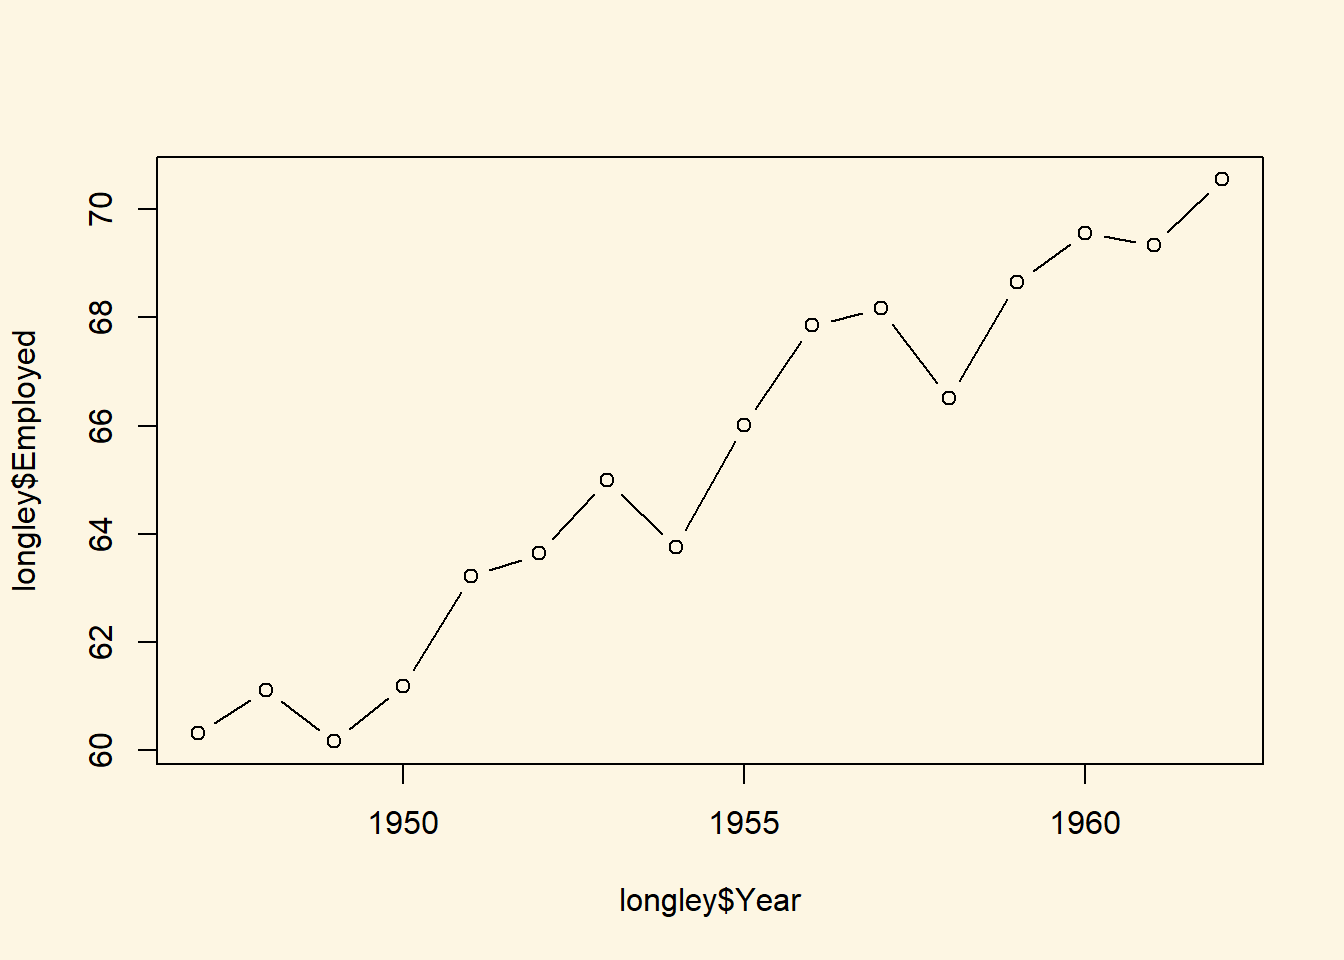
\includegraphics{suffolk2019_files/figure-latex/unnamed-chunk-98-1.pdf}

\hypertarget{correlations-and-differences-in-means}{%
\section{Correlations and differences in means}\label{correlations-and-differences-in-means}}

\hypertarget{seminar-6}{%
\subsection{Seminar}\label{seminar-6}}

Will be uploaded tomorrow

\hypertarget{regression}{%
\section{Regression}\label{regression}}

\hypertarget{seminar-7}{%
\subsection{Seminar}\label{seminar-7}}

Will be uploaded tomorrow

\hypertarget{prediction-and-assessing-prediction-accuracy}{%
\section{Prediction and assessing prediction accuracy}\label{prediction-and-assessing-prediction-accuracy}}

\hypertarget{seminar-8}{%
\subsection{Seminar}\label{seminar-8}}

Will be uploaded tomorrow


\end{document}
